\documentclass[first=dgreen,second=purple,logo=yellowexc]{aaltoslides}
 
\usepackage{xltxtra,xunicode}
\usepackage{fontspec}
\usepackage{verbatim}
\usepackage{bm}
\usepackage{hyperref}
\usepackage{subfig}
\usepackage{caption}
\usepackage{graphicx}

\usepackage[citestyle=authoryear,backend = biber]{biblatex}
\addbibresource{multiplicative-nerv-ref.bib}
 
\setmainfont[Mapping=tex-text]{Linux Libertine O}
\setmonofont{Consolas}
\setsansfont{Constantia}

%\usepackage[T1]{fontenc}


\title{Multiplicative Update For Fast Optimization of Information Retrieval Based Neighbor Embedding}
\author{Jaakko Peltonen, Ziyuan Lin}\date{\today}
\institute[ICS]{Department of Information and Computer Science\\
Aalto University}

\DeclareMathOperator*{\argmin}{arg\,min\,}
\DeclareMathOperator*{\argmax}{arg\,max\,}

\begin{document}

\aaltotitleframe

\begin{frame}{Outline}
\tableofcontents
\end{frame}

\begin{frame}{Summary}
\begin{enumerate}
\item \emph{Neighbor Retrieval Visualizer} (NeRV) is the first non-linear dimensional reduction method that formulates dimensional reduction as an information retrieval task. It directly optimizes information retrieval measures which makes it outperform other non-linear dimension reduction methods;
\item We propose a multiplicative update rule for the NeRV which makes it faster and preserve the good quality as the original NeRV method;
\end{enumerate}
\end{frame}

\section{Neighbor retrieval visualizer}

\begin{frame}{An Example of NeRV}
\begin{figure}
\captionsetup[subfigure]{labelformat=empty}
\centering
\begin{tabular}{ccc}
\subfloat[A 3D sphere]{\includegraphics[width=0.3\textwidth]{figures/glyphsphere1c.eps}} & 
\subfloat["Tearing-open"]{\includegraphics[width=0.3\textwidth]{figures/glyphsphere-2d-l0.pdf}} &
\subfloat["Squashing"]{\includegraphics[width=0.3\textwidth]{figures/glyphsphere-2d-l1.pdf}} 
\end{tabular}
\caption{Two ways showing 2D visualizations of a sphere: \textbf{A}) to tear it open, which emphasizes precision; or \textbf{B}) to squash it flat, which emphasizes recall.}
\end{figure}
\end{frame}

\begin{frame}{Errors in visual information retrieval}
\begin{figure}
\centering
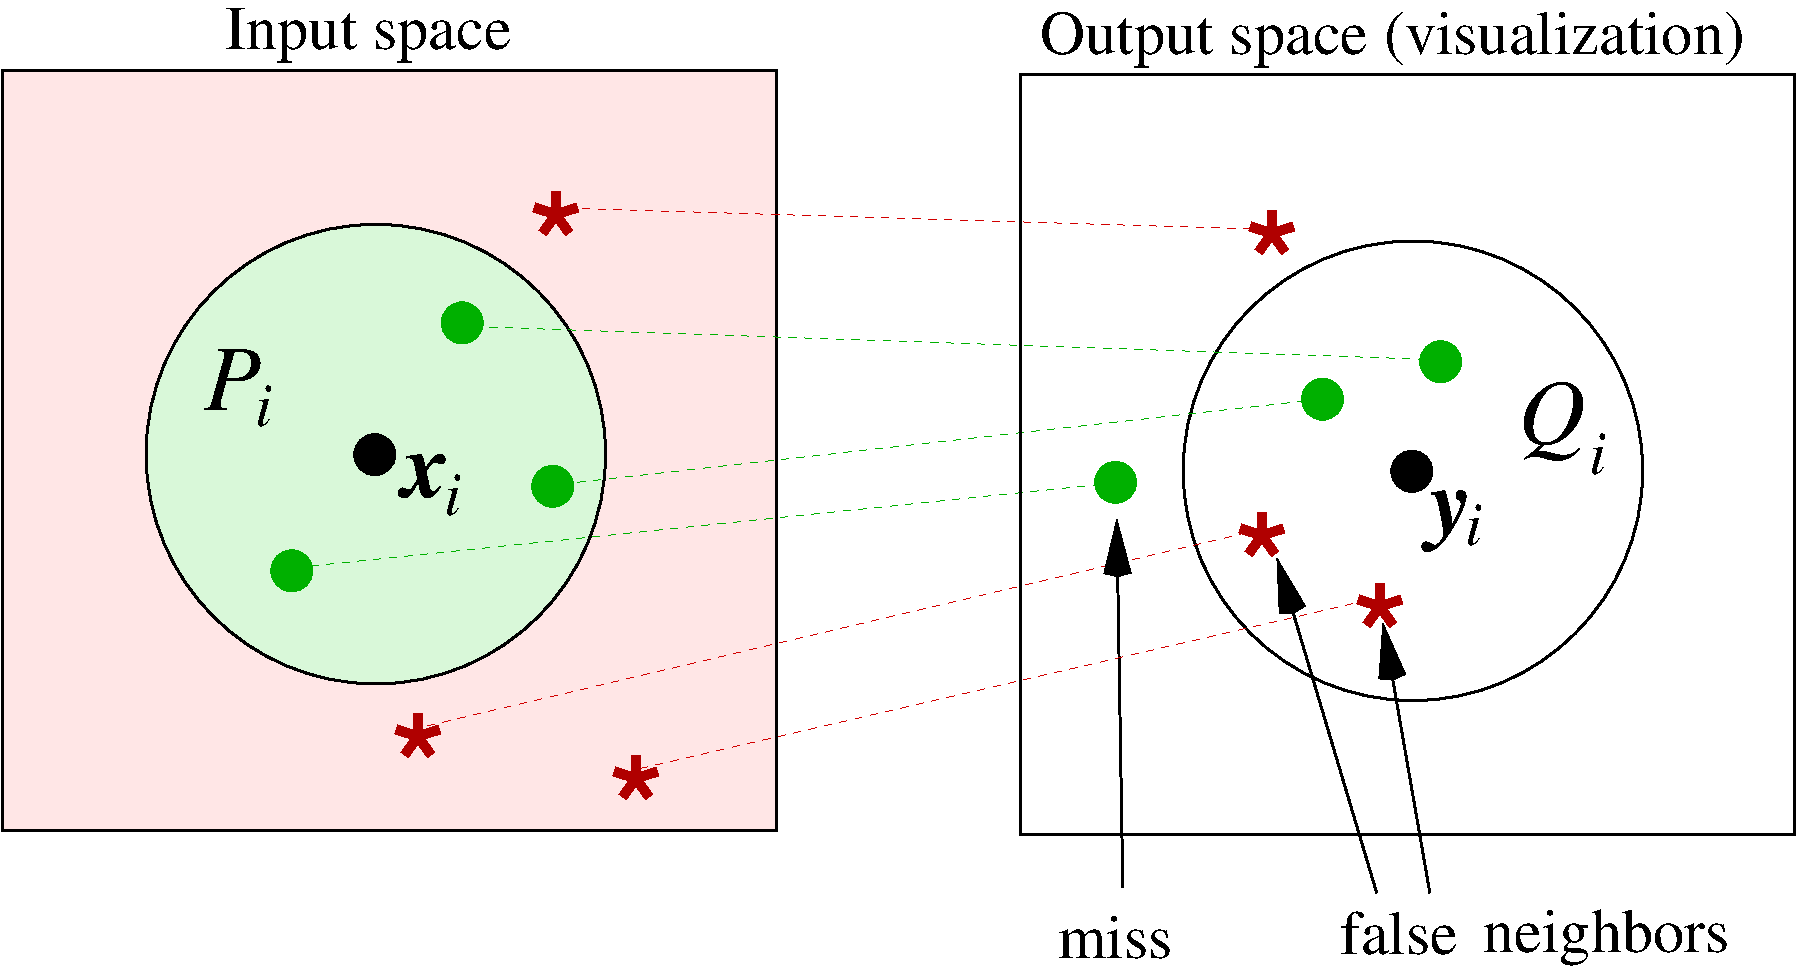
\includegraphics[width=\textwidth]{figures/retrieval_illustration.pdf}
\caption{\footnotesize{\emph{Misses} are true neighbors that are not neighbors on the display; \emph{false neighbors} are neighbors on the display that are not true neighbors.}}
\end{figure}
\end{frame}

\begin{frame}{Technical detail of NeRV}
The resulting total cost of errors turns out to be KL-divergences between neighborhood distributions (\cite{venna10jmlr}):
\begin{align*}
\{y^*_{ij}\}=&\argmin_{\{y_{ij}\}}\sum_i\sum_{j\ne i}\lambda p_{ij}\log\frac{p_{ij}}{q_{ij}}+(1-\lambda)q_{ij}\log\frac{q_{ij}}{p_{ij}}\\
\triangleq &\argmin_{\{y_{ij}\}}\sum_i\lambda KL(P_i\|Q_i)+(1-\lambda)KL(Q_i\|P_i)
\end{align*}
where
\[
p_{ij} = \frac{\exp(-d(x_i,x_j)^2/(2\sigma^2_i))}{\sum_{k\ne i} \exp(-d(x_i,x_k)^2)/(2\sigma^2_i)},\;
q_{ij} = \frac{\exp(-\|y_i-y_j\|^2/(2\sigma^2_i))}{\sum_{k\ne i} \exp(-\|y_i-y_k\|^2)/(2\sigma^2_i)}
\]

\[
KL(P_i\|Q_i)\propto \mbox{ \#misses},\;KL(Q_i\|P_i)\propto \mbox{ \#false neighbors}
\]

\end{frame}


\section{How to make it fast}
\begin{frame}{NeRV is slow}

NeRV is based on the traditional gradient descent method, which uses the additive update rule that needs a line search for the step size $\alpha$:
\[
z^{(t+1)}_{id}=z^{(t)}_{id}-\alpha_{id} \nabla_{id} \mathcal{J}(z^{(t)})\;,
\]
where
\begin{align*}
z^{(t)}_{id}:&\mbox{ the $(i,d)$-th parameter at the $t$-th iteration;}\\
\mathcal{J}:&\mbox{ the cost function;}\\
\nabla_{id}:&\mbox{ the $(i,d)$-th component of the gradient;}
\end{align*}
\end{frame}

\begin{frame}{NeRV is slow}
\begin{itemize}
\item This additive rule is widely used, but it is slow in cases that need fast response. For example the user interaction application (\cite{peltonen13eurovis}) of NeRV that we have explored recently;
\item The Quad-tree based accelerations (\cite{yang13icml} or \cite{vandermaaten13iclr}) are comparable methods, but they have to assume the neighborhood distribution to be sparse, while what we present here has no such requirements.
\end{itemize}
\end{frame}

\begin{frame}{Our method}
To avoid the tuning or line search in the additive update, we derive the \emph{multiplicative} update rule as below. The work in (\cite{yang10mlsp}) is a special case for t-SNE.
\[
z^{(t+1)}_{id}=z^{(t)}_{id}\frac{\nabla^-_{id} \mathcal{J}(z^{(t)})}{\nabla^+_{id} \mathcal{J}(z^{(t)})}\;,
\]
where $\nabla_{id}^+$ and $\nabla_{id}^-$ is a decomposition of the gradient that satisfies
\begin{align*}
\nabla_{id}\mathcal{J} =& \nabla_{id}^+\mathcal{J}-\nabla_{id}^-\mathcal{J}\\
\nabla_{id}^+\mathcal{J} \ge& 0\\
\nabla_{id}^-\mathcal{J} \ge& 0
\end{align*}
\end{frame}

\begin{frame}{Connections with additive update}
\begin{enumerate}
\item They have the same extreme points:
\begin{align*}
& z_{id}^{(t+1)}=z_{id}^{(t)} \mbox{ (in additive update)}\\
\Longrightarrow& \nabla_{id}\mathcal{J}(z_{id})=0\\
\Longrightarrow& \nabla_{id}^+\mathcal{J}(z_{id})=\nabla_{id}^-\mathcal{J}(z_{id})\\
\Longrightarrow& z_{id}^{(t+1)}=z_{id}^{(t)}\mbox{ (in multiplicative update)}
\end{align*}
\item
\[
\left.
\begin{aligned}
z^{(t+1)}_{id} =& z^{(t)}_{id}-\alpha_{id} \nabla_{id} \mathcal{J}(z^{(t)})\\
\alpha_{id} =& \frac{z_{id}^{(t)}}{\nabla_{id}^+\mathcal{J}(z_{id}^{(t)})}
\end{aligned}
\right\}\Longrightarrow z^{(t+1)}_{id}=z^{(t)}_{id}\frac{\nabla^-_{id} \mathcal{J}(z^{(t)})}{\nabla^+_{id} \mathcal{J}(z^{(t)})}
\]
\end{enumerate}
\end{frame}


\begin{frame}{The pipeline of multiplicative NeRV}
\begin{enumerate}
\item The multiplicative update rule is sign preserving. So we transform the coordinates with $z_{id}^{(0)}=\exp(y_{id}^{(0)})$;
\item Update multiplicatively
\[
z^{(t+1)}_{id}=z^{(t)}_{id}\frac{\nabla^-_{id} \mathcal{J}(z^{(t)})}{\nabla^+_{id} \mathcal{J}(z^{(t)})}
\]
for a sufficient number of iterations. In our experiments, 300 iterations works empirically well;
\item Transform back to the display space:
\[
y_{id}^* =\log z^{*}_{id}
\]
\end{enumerate}
\end{frame}

\begin{frame}{Information retrieval perspective interpretation}
\begin{itemize}
\item The  multiplicative rule is that it is intuitive understandable, because terms in update rule have information retrieval interpretation;
\item It pushes the coordinates $y_{id}$ away from the worst false neighbors of $i$ and towards missed neighbors;
\item More details are available in the paper.
\end{itemize}
\end{frame}

\section{Experiments}
\begin{frame}{Experiments}
Our experiments show three things: 
\begin{enumerate}
\item Our update rule produces visually similar results as the original NeRV;
\item It improves much faster;
\item In quantitative comparison, it outperforms many earlier methods.
\end{enumerate}
\end{frame}


\begin{frame}{Experiments: results on Plain S-curve}
\begin{figure}[!htb]
\captionsetup[subfigure]{labelformat=empty}
\centering
\begin{tabular}{cc}
\subfloat[Multiplicative]{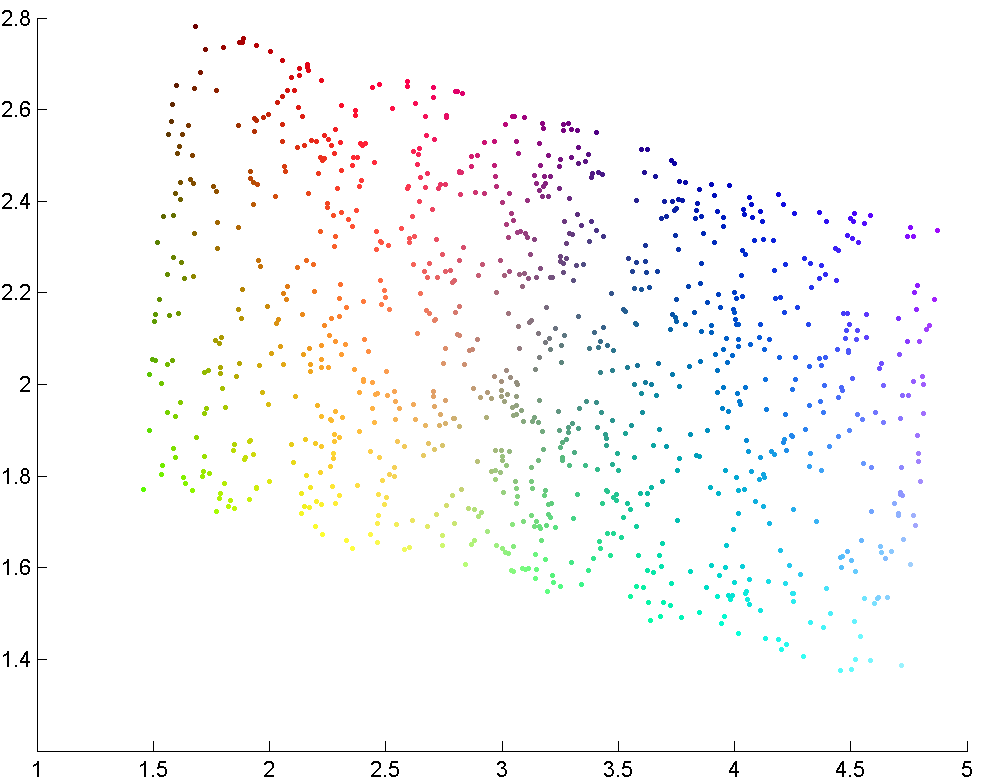
\includegraphics[height=0.5\textheight]{figures/s-data-0-nerv-0_1.pdf}} & 
\subfloat[Additive]{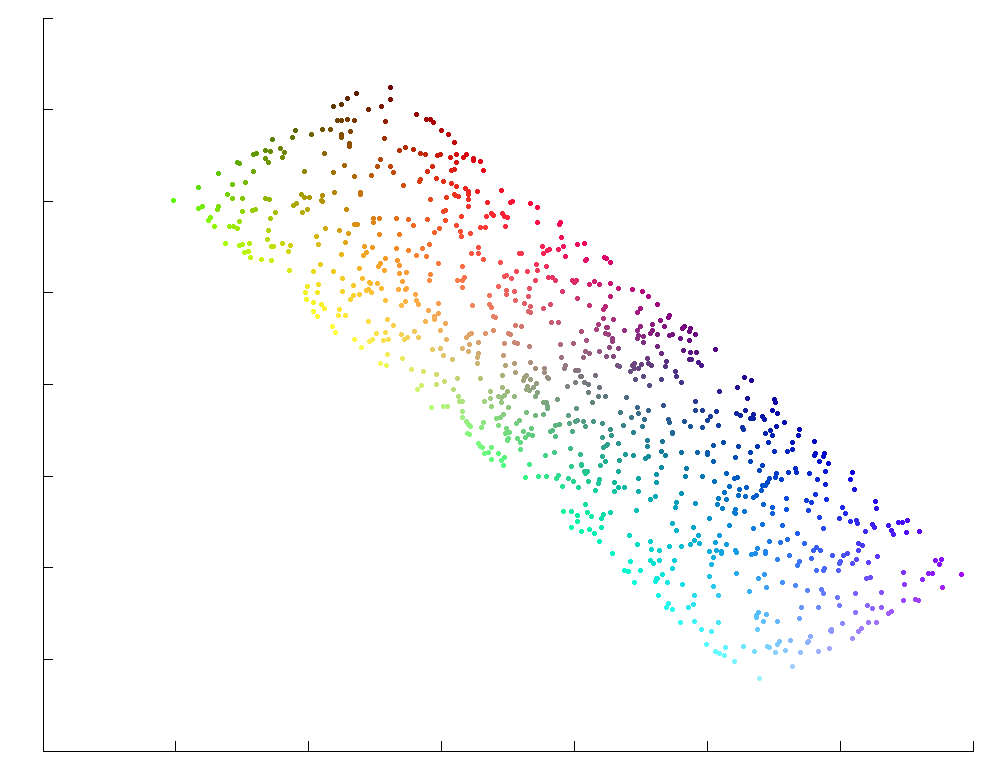
\includegraphics[height=0.5\textheight]{figures/s-data-0-original-nerv-0_1.pdf}}\\
\end{tabular}
\caption{Colors correspond to original 3D coordinates.}
\end{figure}
\end{frame}


\begin{frame}{Experiments: results on Sphere}
\begin{figure}[!htb]
\captionsetup[subfigure]{labelformat=empty}
\centering
\begin{tabular}{cc}
\subfloat[Multiplicative]{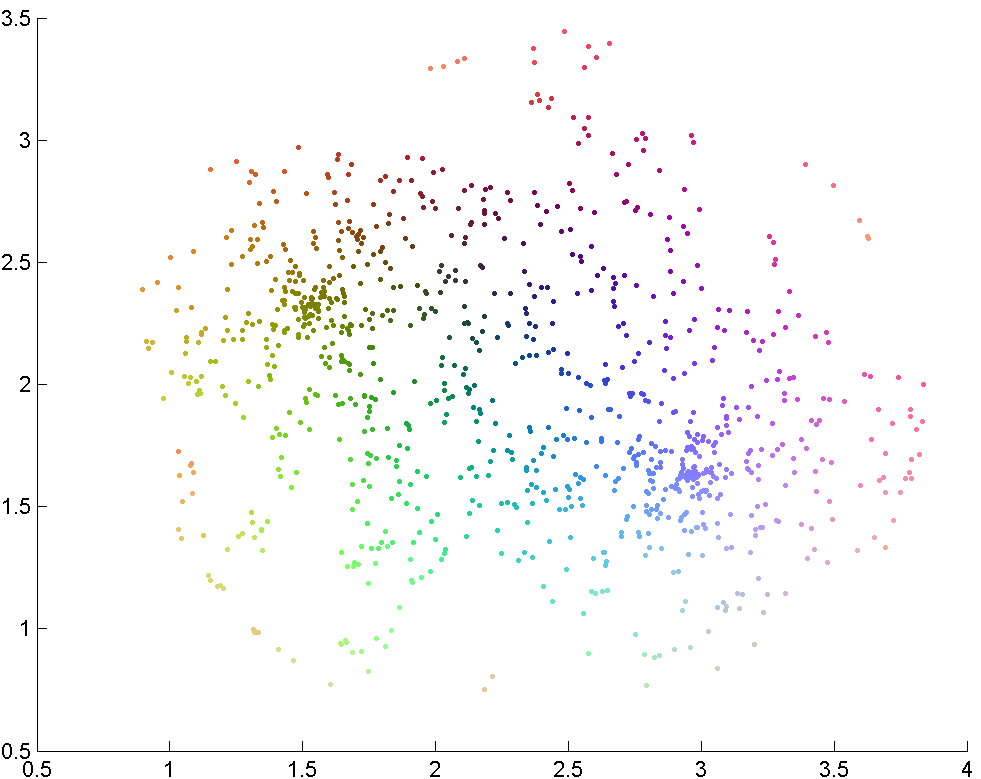
\includegraphics[height=0.5\textheight]{figures/sphere-nerv-0_1.pdf}} &
\subfloat[Additive]{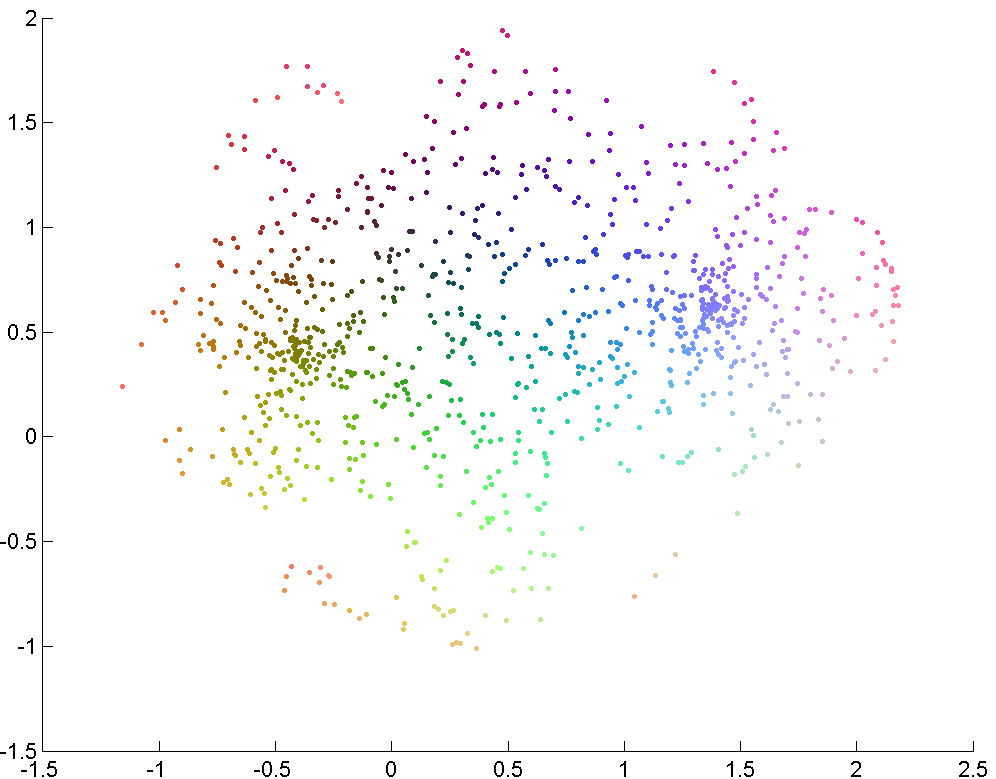
\includegraphics[height=0.5\textheight]{figures/sphere-original-nerv-0_1.pdf}}
\end{tabular}
\caption{Colors correspond to original 3D coordinates.}
\end{figure}
\end{frame}


\begin{frame}{Experiments: results on Phoneme}
\begin{figure}[!htb]
\captionsetup[subfigure]{labelformat=empty}
\centering
\begin{tabular}{cc}
\subfloat[Multiplicative]{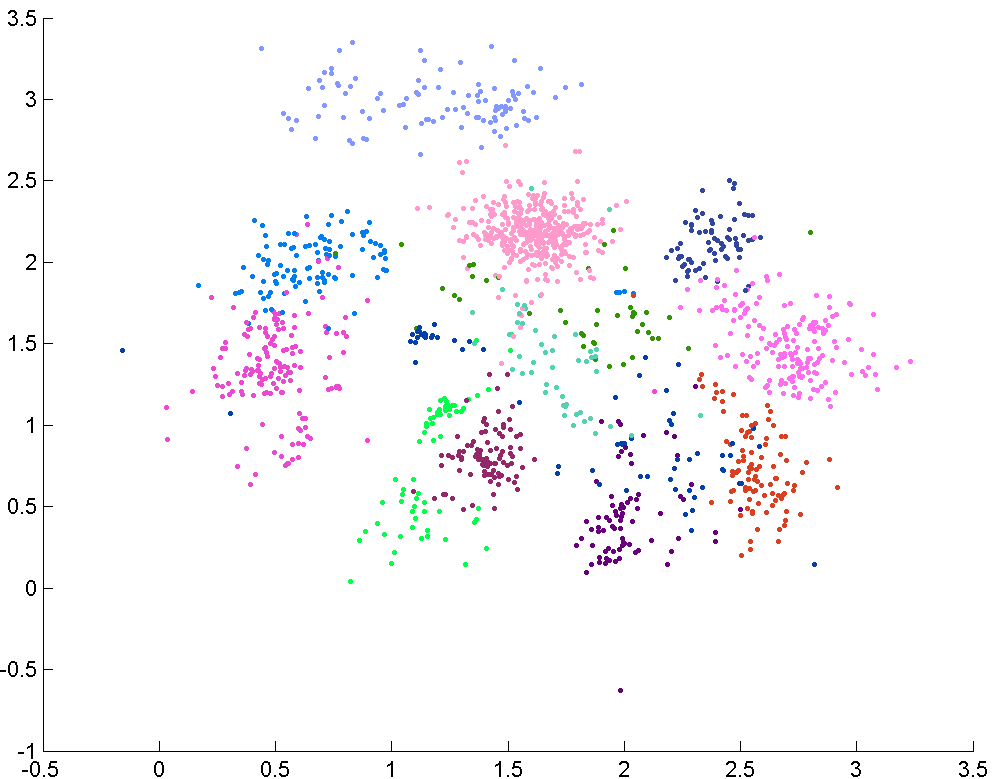
\includegraphics[height=0.5\textheight]{figures/lvqdata-nerv-0_1.pdf}} &
\subfloat[Additive]{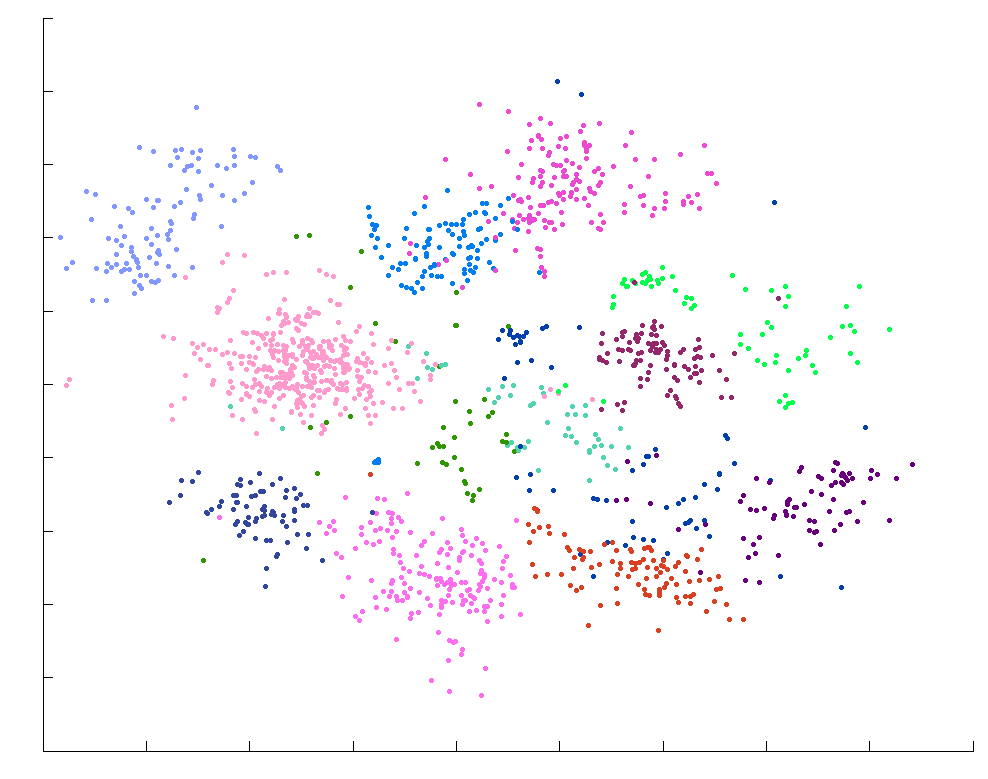
\includegraphics[height=0.5\textheight]{figures/lvqdata-original-nerv-0_1.pdf}}
\end{tabular}
\caption{A data set of phonemes (very short audio samples for speech). Colors correspond to different phonemes.}
\end{figure}
\end{frame}


\begin{frame}{Experiments: results on Landsat}
\begin{figure}[!htb]
\captionsetup[subfigure]{labelformat=empty}
\centering
\begin{tabular}{cc}
\subfloat[Multiplicative]{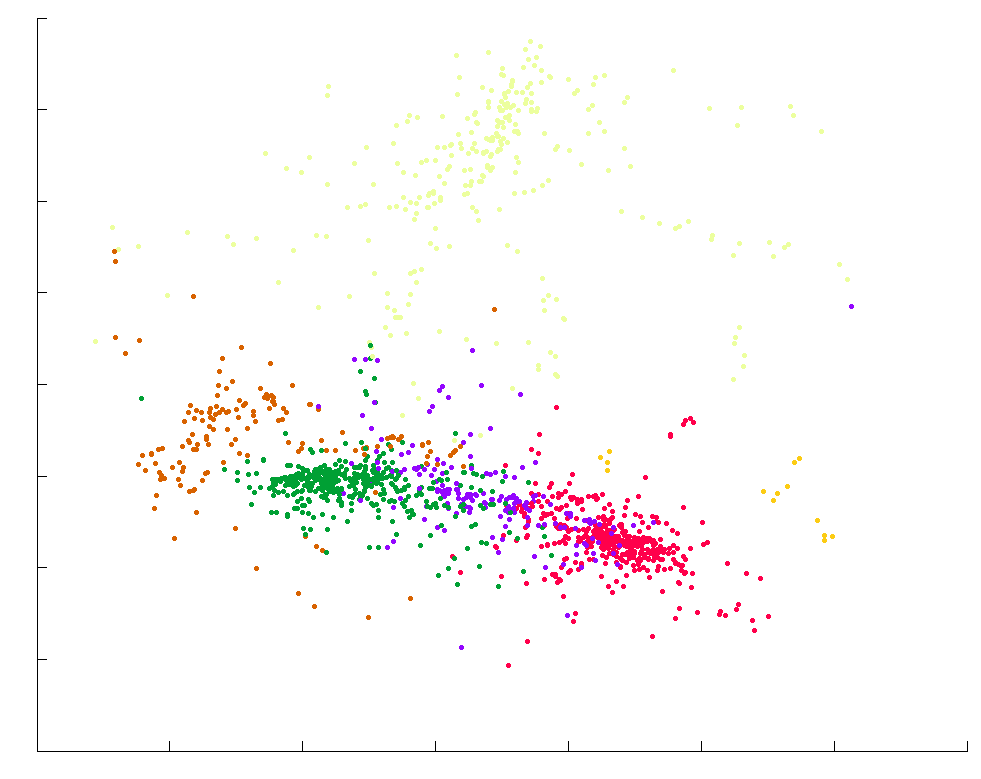
\includegraphics[height=0.5\textheight]{figures/landsat-nerv-0_1.pdf}} &
\subfloat[Additive]{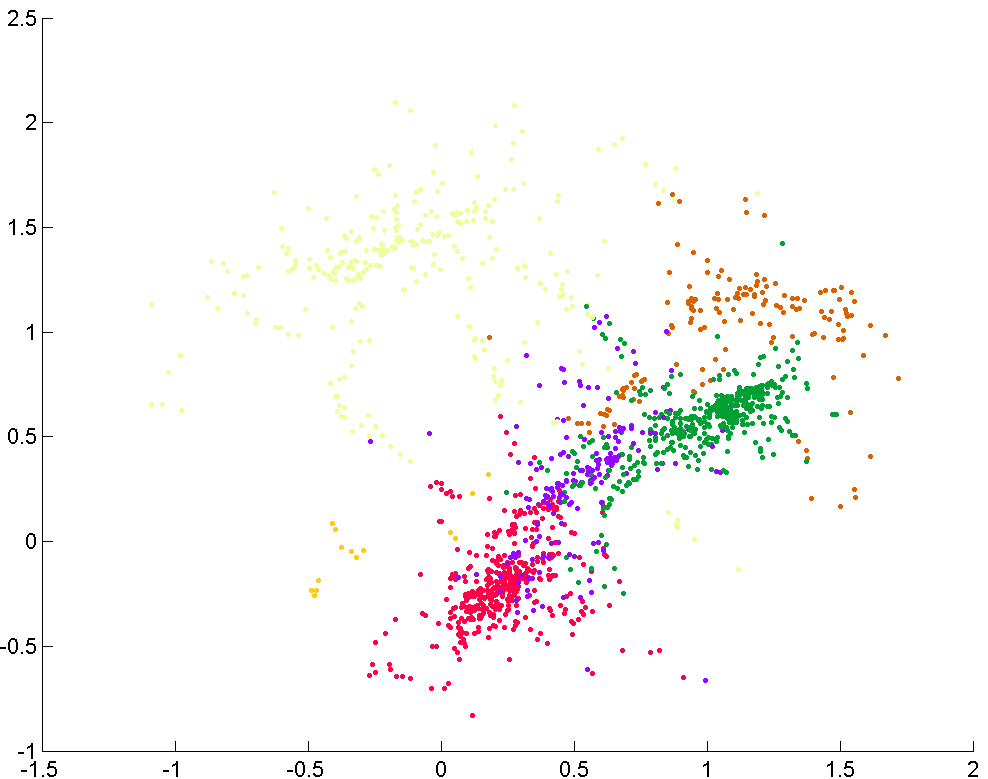
\includegraphics[height=0.5\textheight]{figures/landsat-original-nerv-0_1.pdf}}
\end{tabular}
\caption{A data set of images of land taken by satellite. Colors correspond to terrain types.}
\end{figure}
\end{frame}


\begin{frame}{Experiments: results on MNIST}
\begin{figure}[!htb]
\captionsetup[subfigure]{labelformat=empty}
\centering
\begin{tabular}{cc}
\subfloat[Multiplicative]{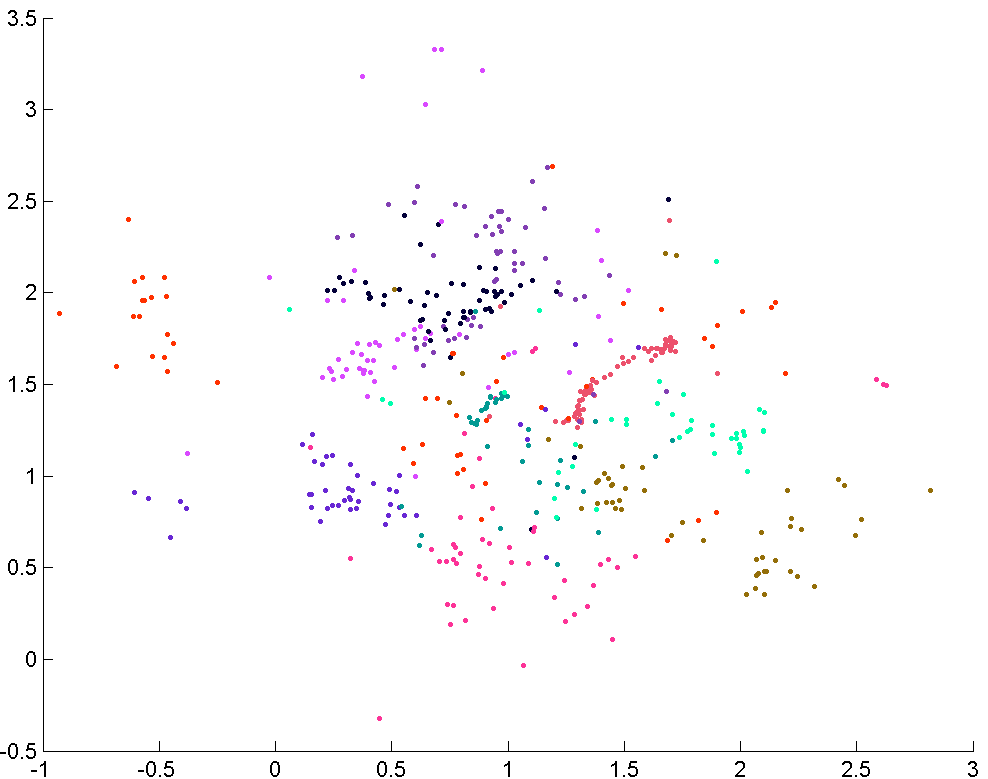
\includegraphics[height=0.5\textheight]{figures/MNIST-500-nerv-0_1.pdf}} &
\subfloat[Additive]{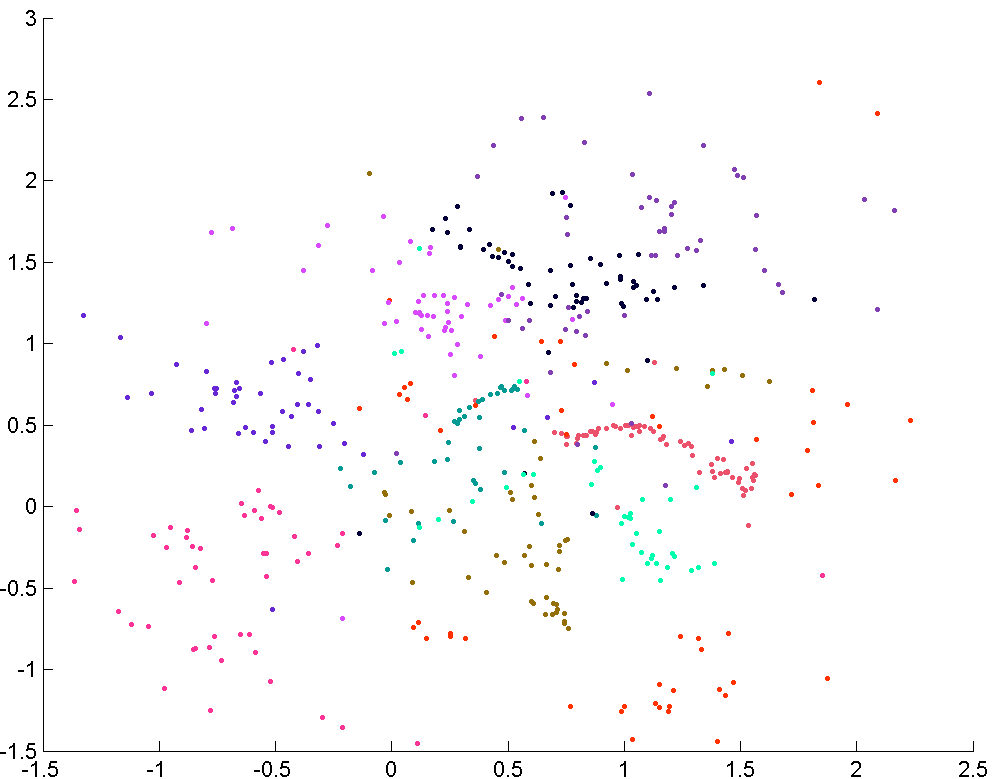
\includegraphics[height=0.5\textheight]{figures/MNIST-500-original-nerv-0_1.pdf}}
\end{tabular}
\caption{A data set for hand-written digits. Colors correspond to different digits.}
\end{figure}
\end{frame}


\begin{frame}{Experiments: results on Olivetti Faces}
\begin{figure}[!htb]
\captionsetup[subfigure]{labelformat=empty}
\centering
\begin{tabular}{cc}
\subfloat[Multiplicative]{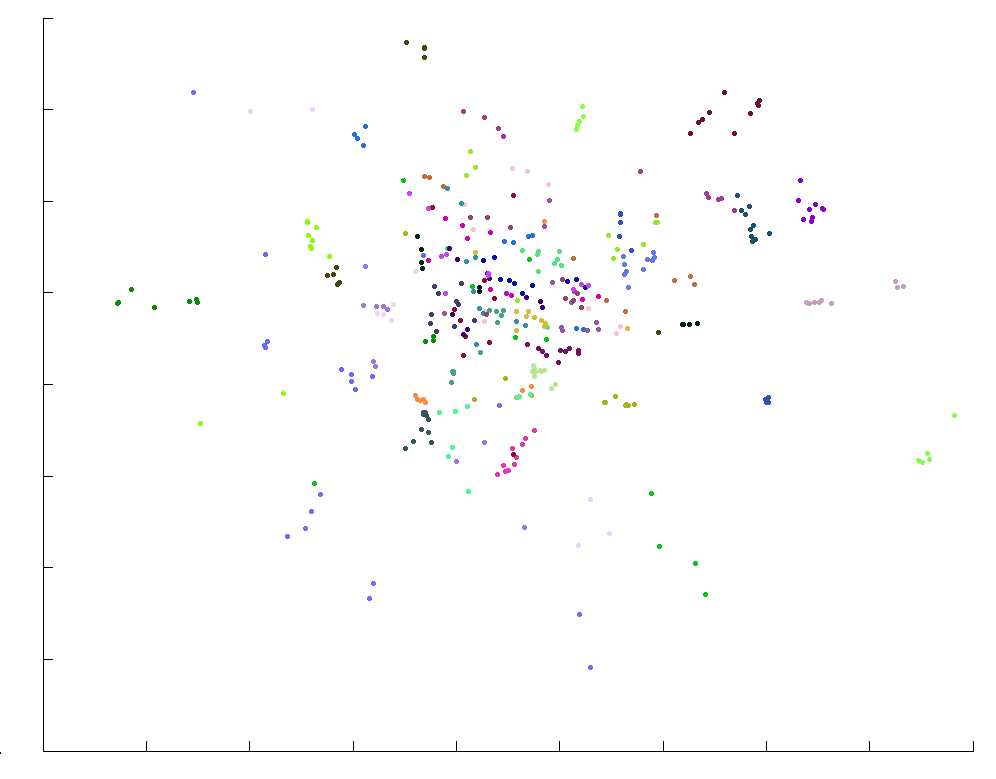
\includegraphics[height=0.5\textheight]{figures/olivettifaces_dist-nerv-0_1.pdf}} &
\subfloat[Additive]{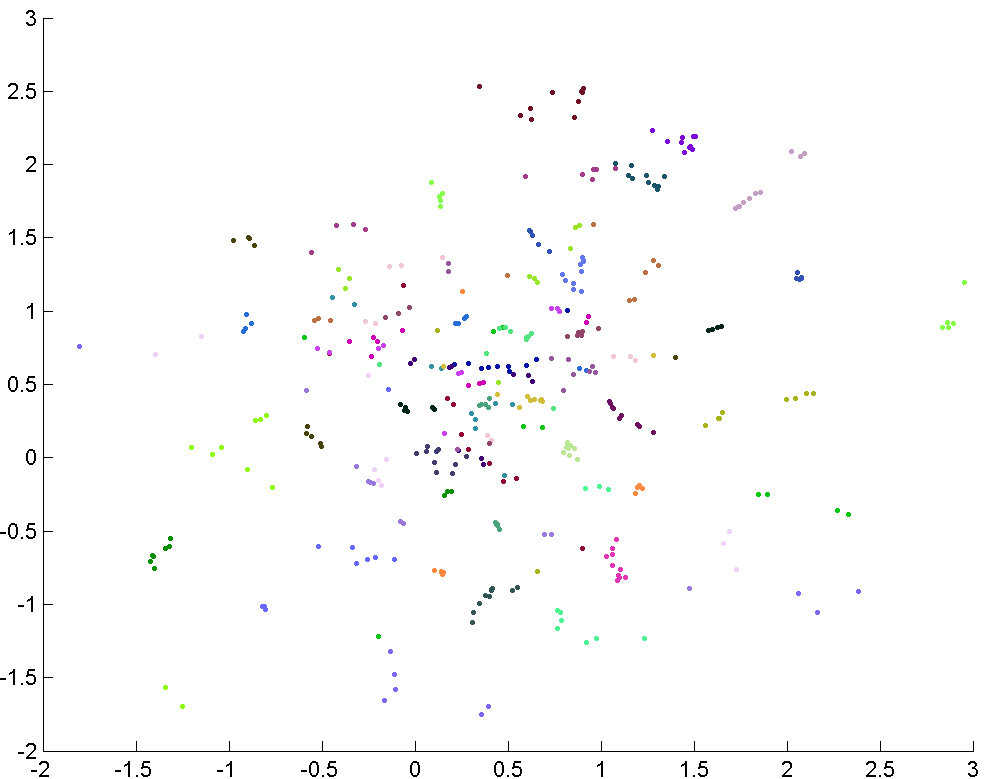
\includegraphics[height=0.5\textheight]{figures/olivettifaces_dist-original-nerv-0_1.pdf}}
\end{tabular}
\caption{A data set of faces. Colors correspond to different people.}
\end{figure}
\end{frame}


\begin{frame}{Experiments: performance}
\begin{figure}[!htb]
\captionsetup[subfigure]{labelformat=empty}
\centering
\begin{tabular}{cc}
\subfloat[Plain S-curve]{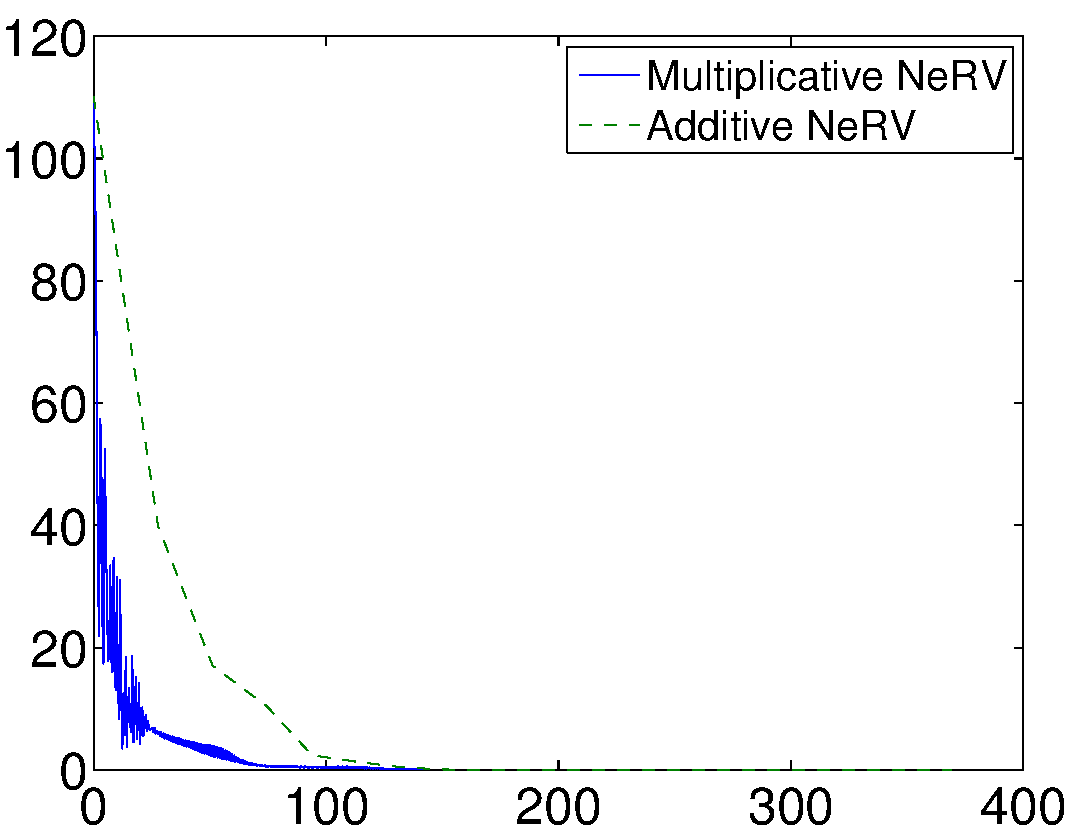
\includegraphics[width=0.5\textwidth]{figures/secs_cost_s-data-0.pdf}} &
\subfloat[Sphere]{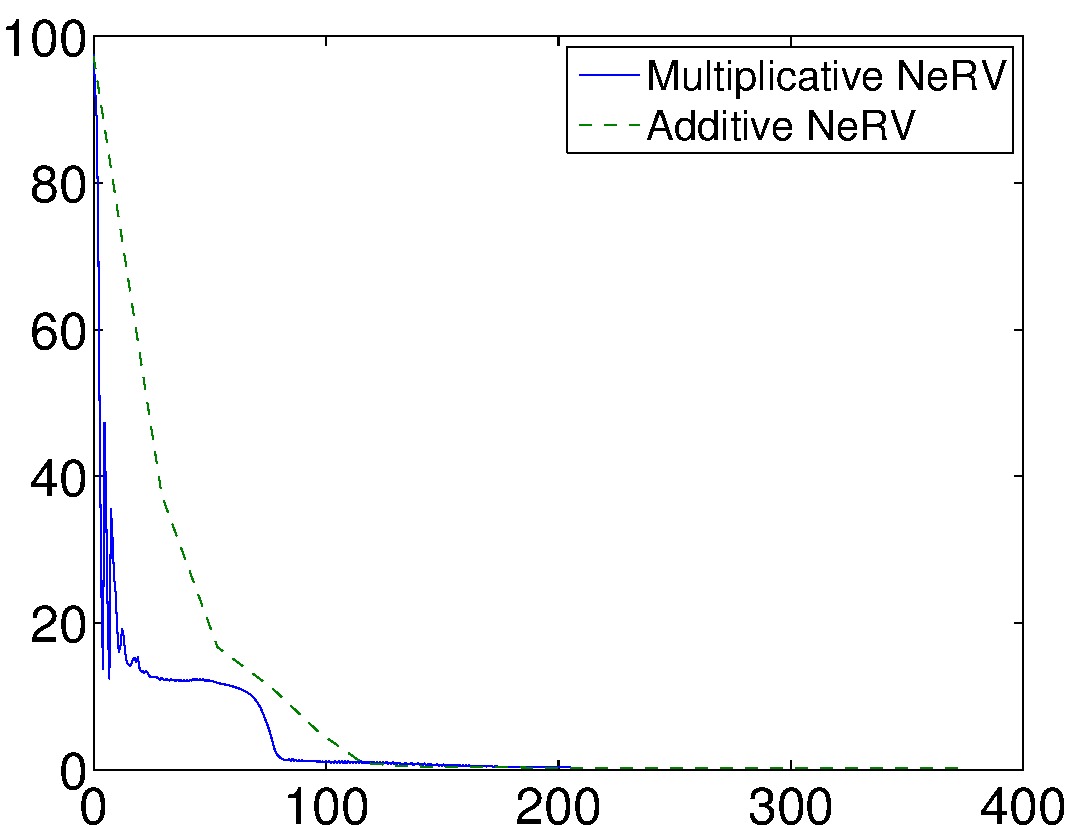
\includegraphics[width=0.5\textwidth]{figures/secs_cost_sphere.pdf}} 
\end{tabular}
\caption{Graphs of running time vs. information retrieval performance (NeRV's cost, the lower the better).}
\end{figure}
\end{frame}


\begin{frame}{Experiments: performance}
\begin{figure}[!htb]
\captionsetup[subfigure]{labelformat=empty}
\centering
\begin{tabular}{cc}
\subfloat[Phoneme]{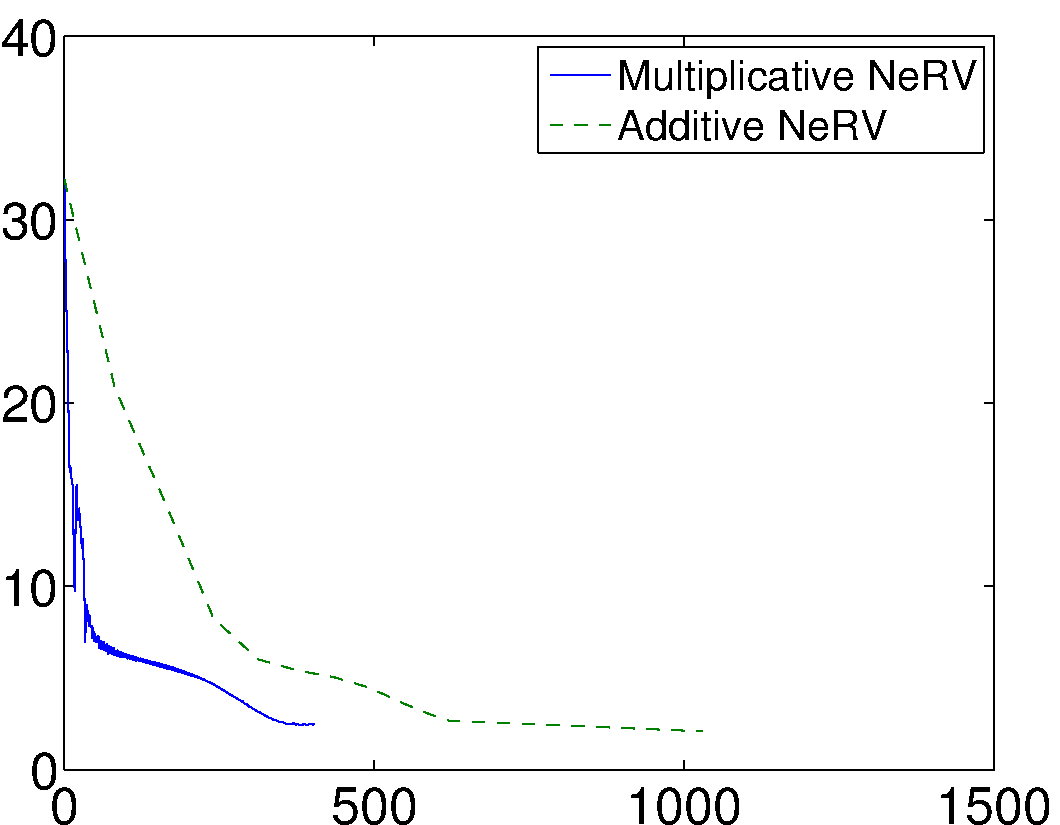
\includegraphics[width=0.5\textwidth]{figures/secs_cost_lvqdata.pdf}} &
\subfloat[Landsat]{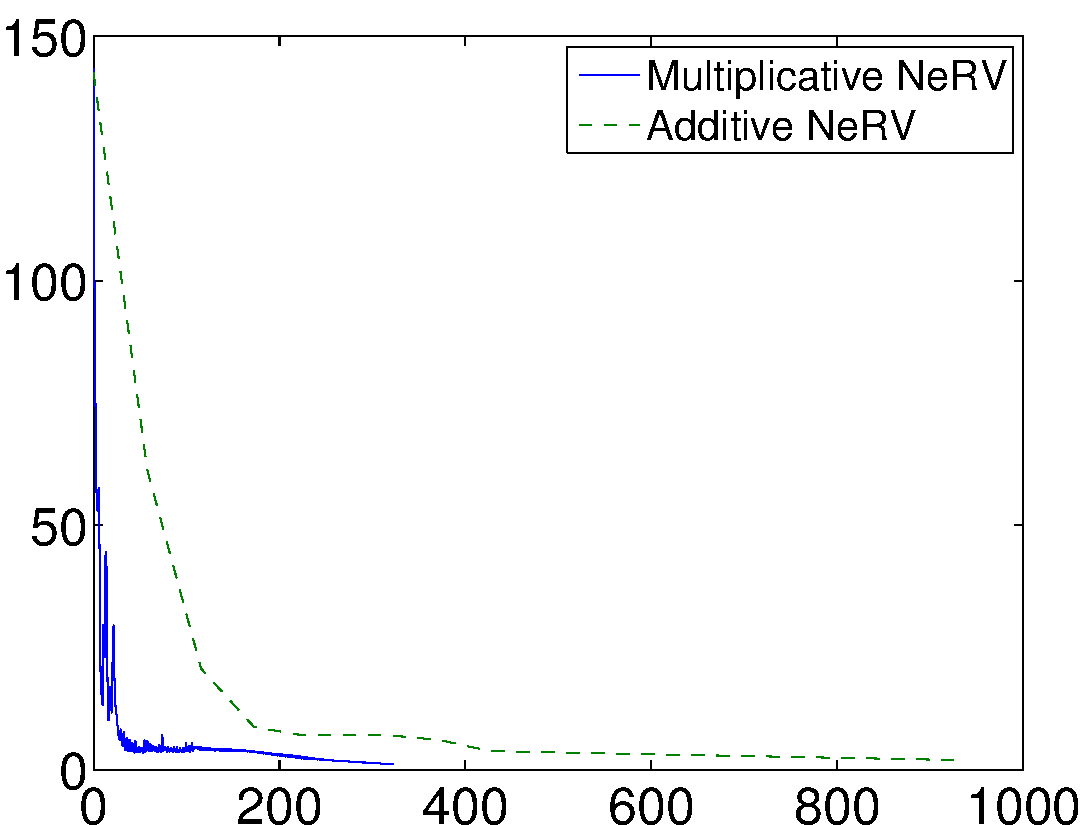
\includegraphics[width=0.5\textwidth]{figures/secs_cost_landsat.pdf}} 
\end{tabular}
\caption{Graphs of running time vs. information retrieval performance (NeRV's cost, the lower the better).}
\end{figure}
\end{frame}


\begin{frame}{Experiments: performance}
\begin{figure}[!htb]
\captionsetup[subfigure]{labelformat=empty}
\centering
\begin{tabular}{cc}
\subfloat[MNIST]{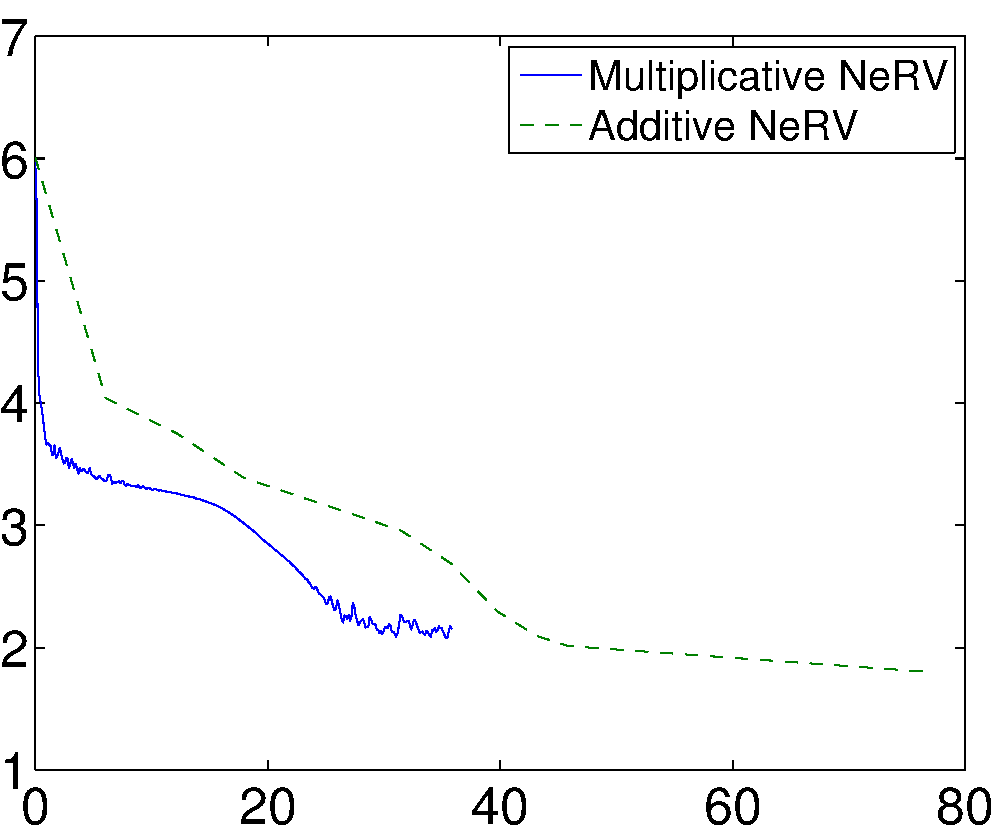
\includegraphics[width=0.5\textwidth]{figures/secs_cost_MNIST-500.pdf}} &
\subfloat[Olivetti Faces]{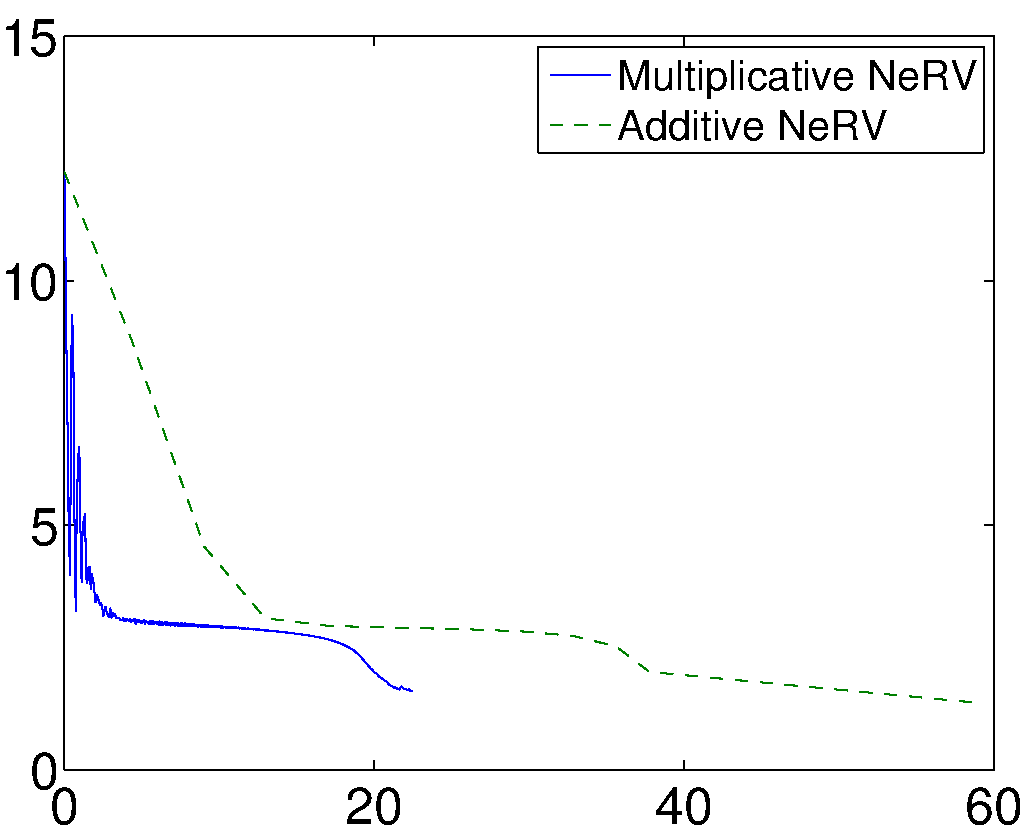
\includegraphics[width=0.5\textwidth]{figures/secs_cost_olivettifaces.pdf}} 
\end{tabular}
\caption{Graphs of running time vs. information retrieval performance (NeRV's cost, the lower the better).}
\end{figure}
\end{frame}


\begin{frame}{Experiments: comparison with other NLDR methods}
\begin{figure}[!htb]
\captionsetup[subfigure]{labelformat=empty}
\centering
\begin{tabular}{cc}
\subfloat[Plain S-curve]{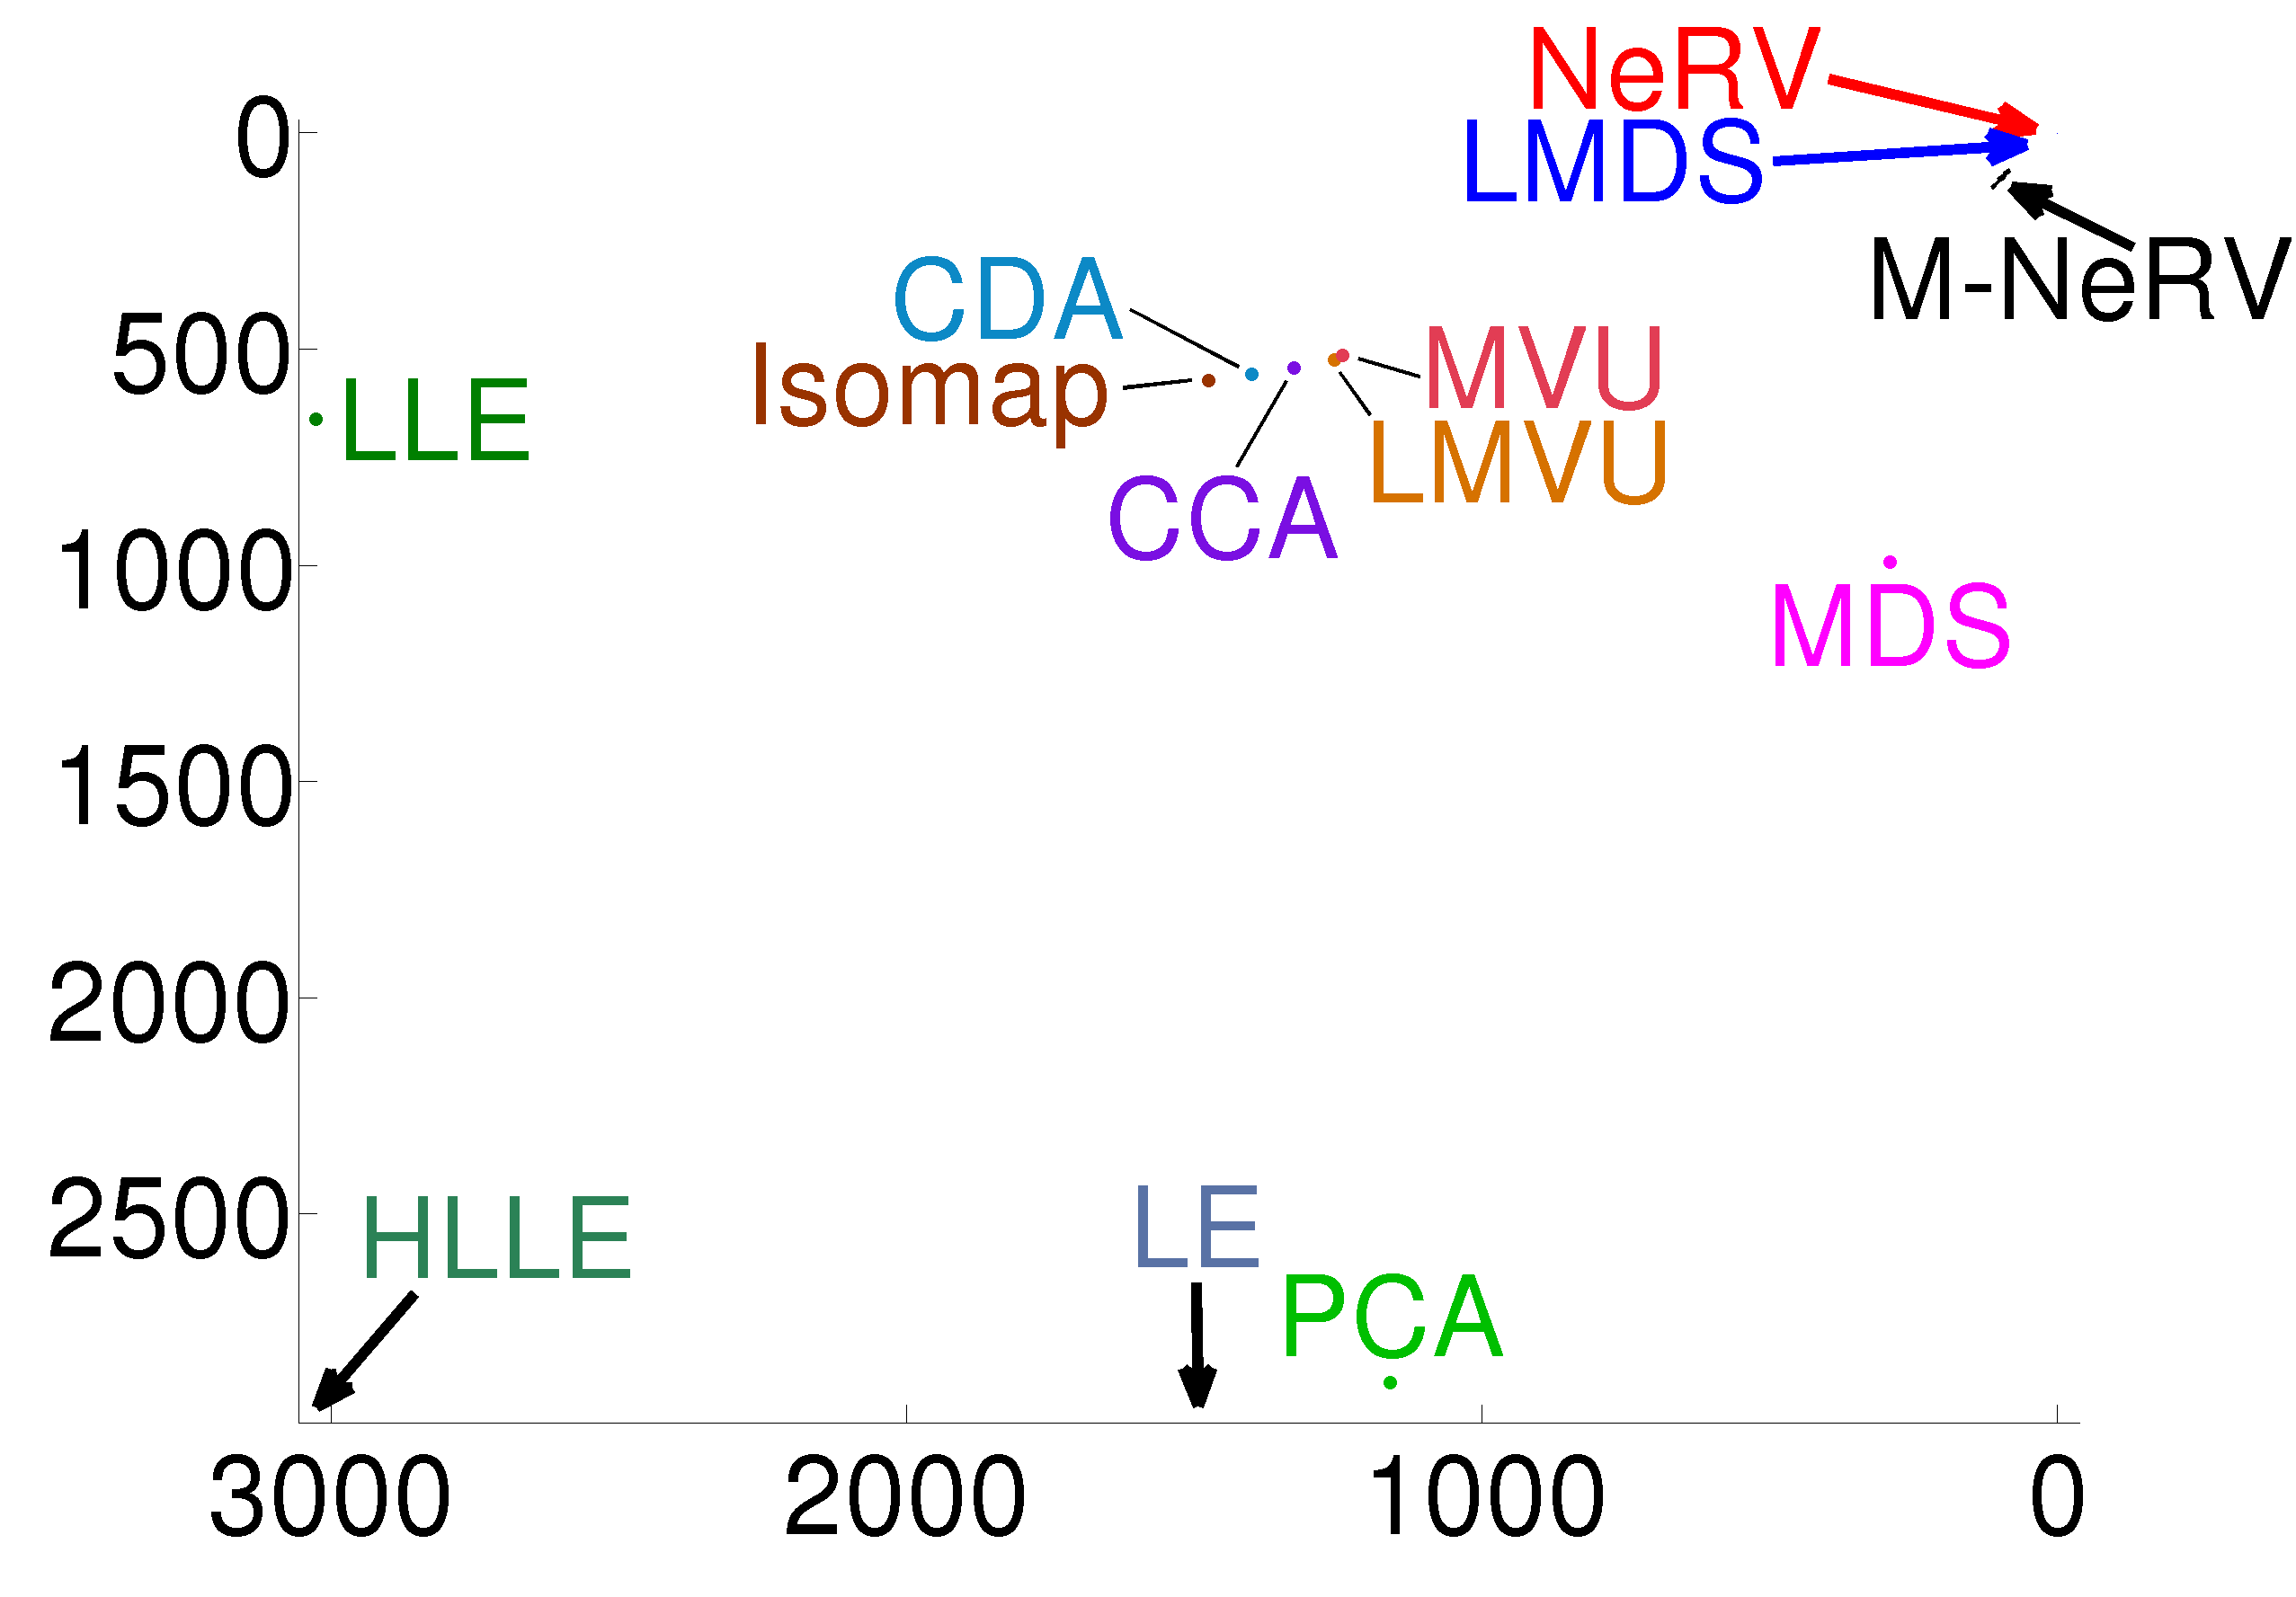
\includegraphics[width=0.5\textwidth]{figures/smoothed-precision-recall-s-data-0.pdf}} &
\subfloat[Noisy S-curve]{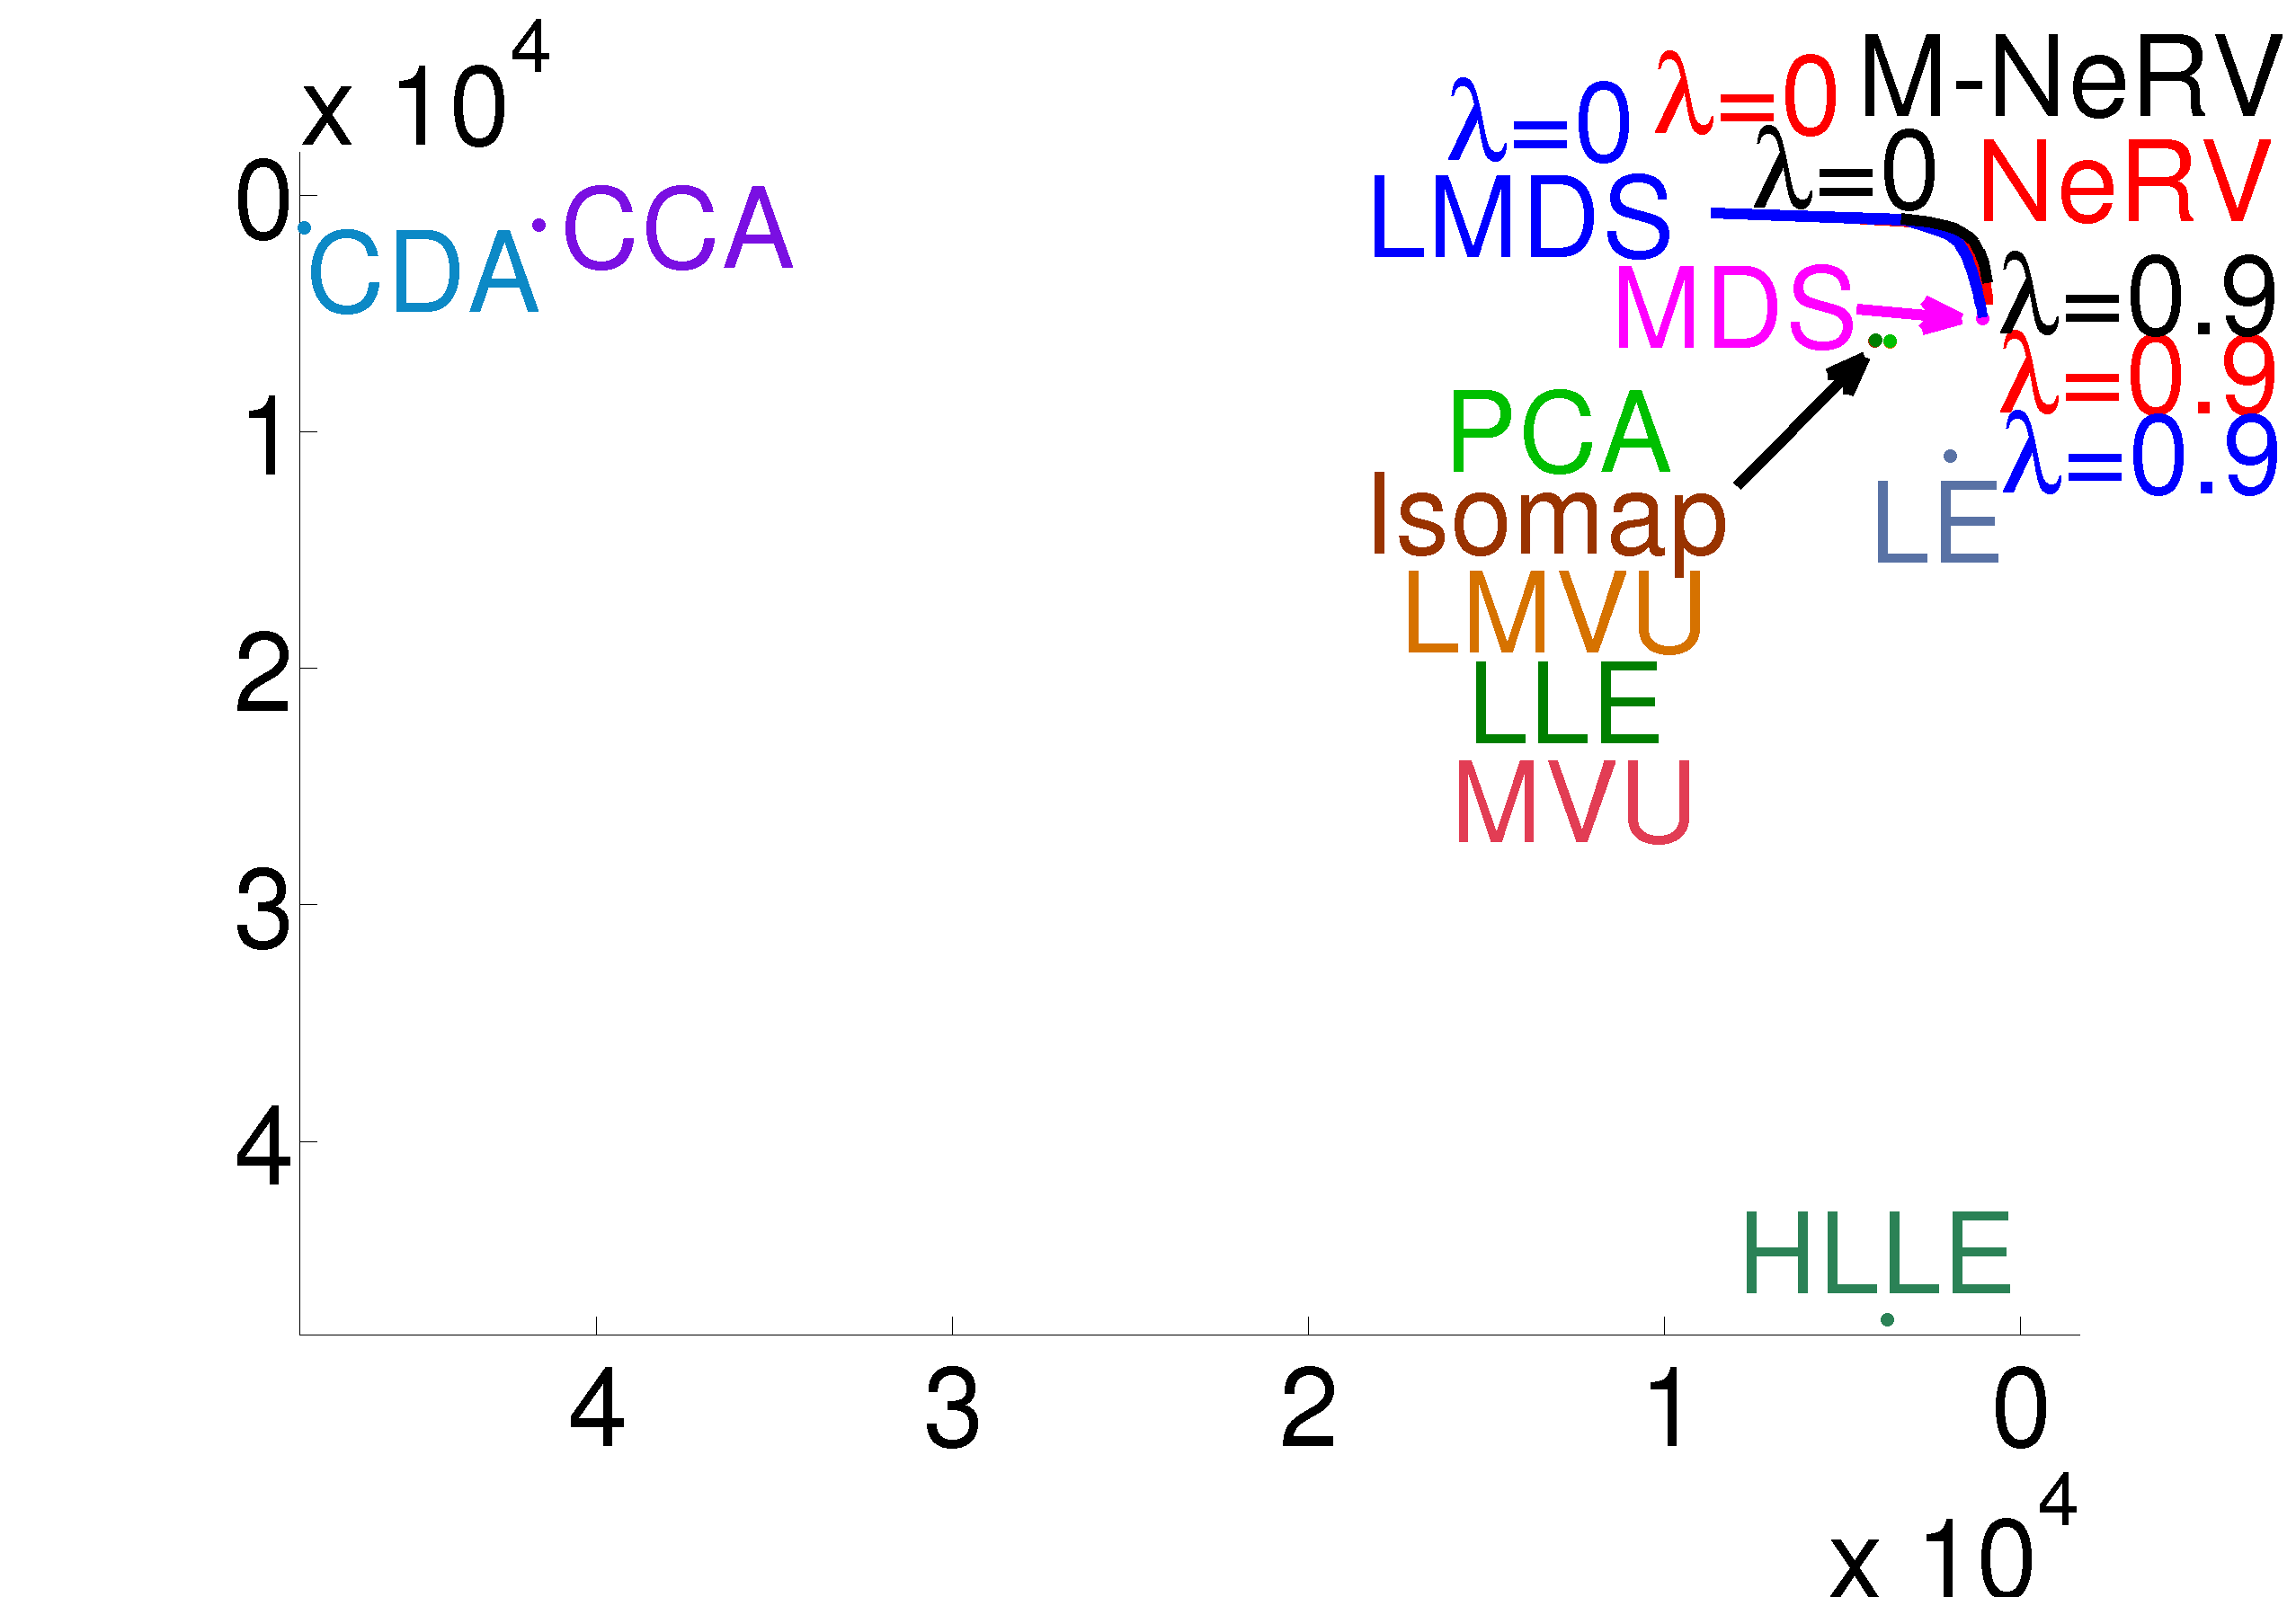
\includegraphics[width=0.5\textwidth]{figures/smoothed-precision-recall-s-data-06.pdf}} 
\end{tabular}
\caption{Mean smoothed recall vs. mean smoothed precision for different methods. Best methods are located top-right.}
\end{figure}
\end{frame}


\begin{frame}{Experiments: comparison with other NLDR methods}
\begin{figure}[!htb]
\captionsetup[subfigure]{labelformat=empty}
\centering
\begin{tabular}{cc}
\subfloat[Olivetti Faces]{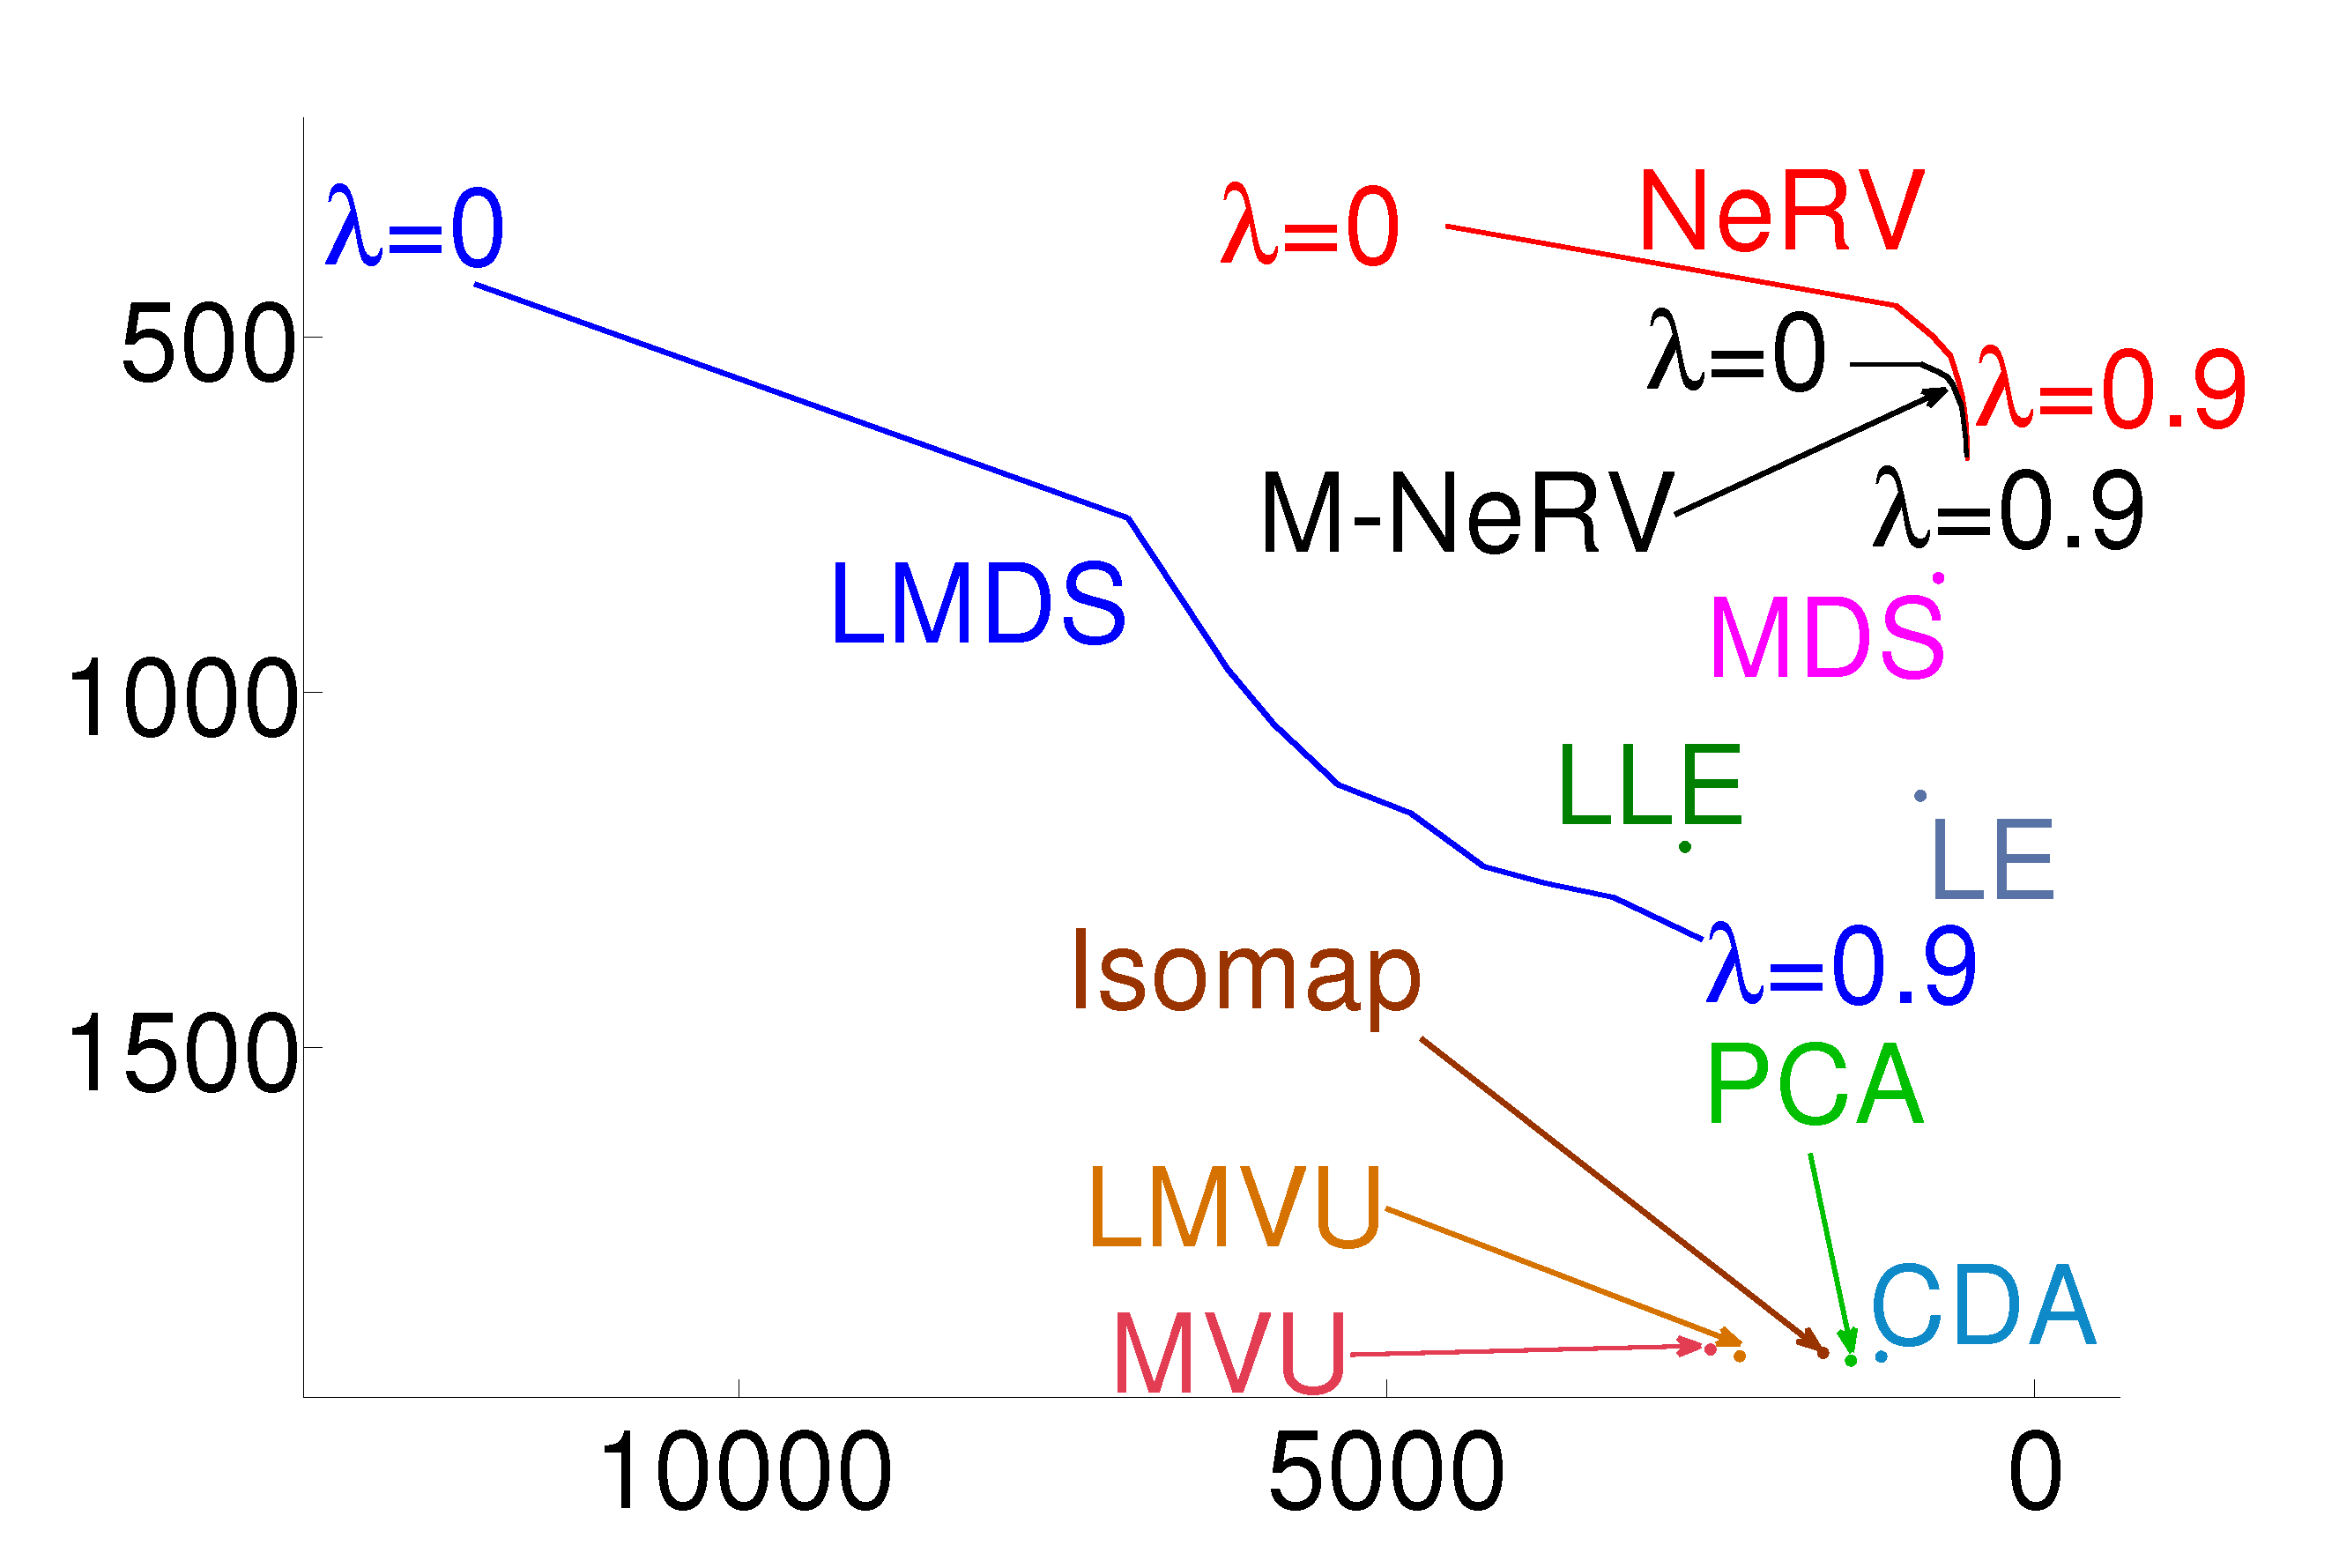
\includegraphics[width=0.5\textwidth]{figures/smoothed-precision-recall-olivettifaces.pdf}} &
\subfloat[Mouse Gene Expression]{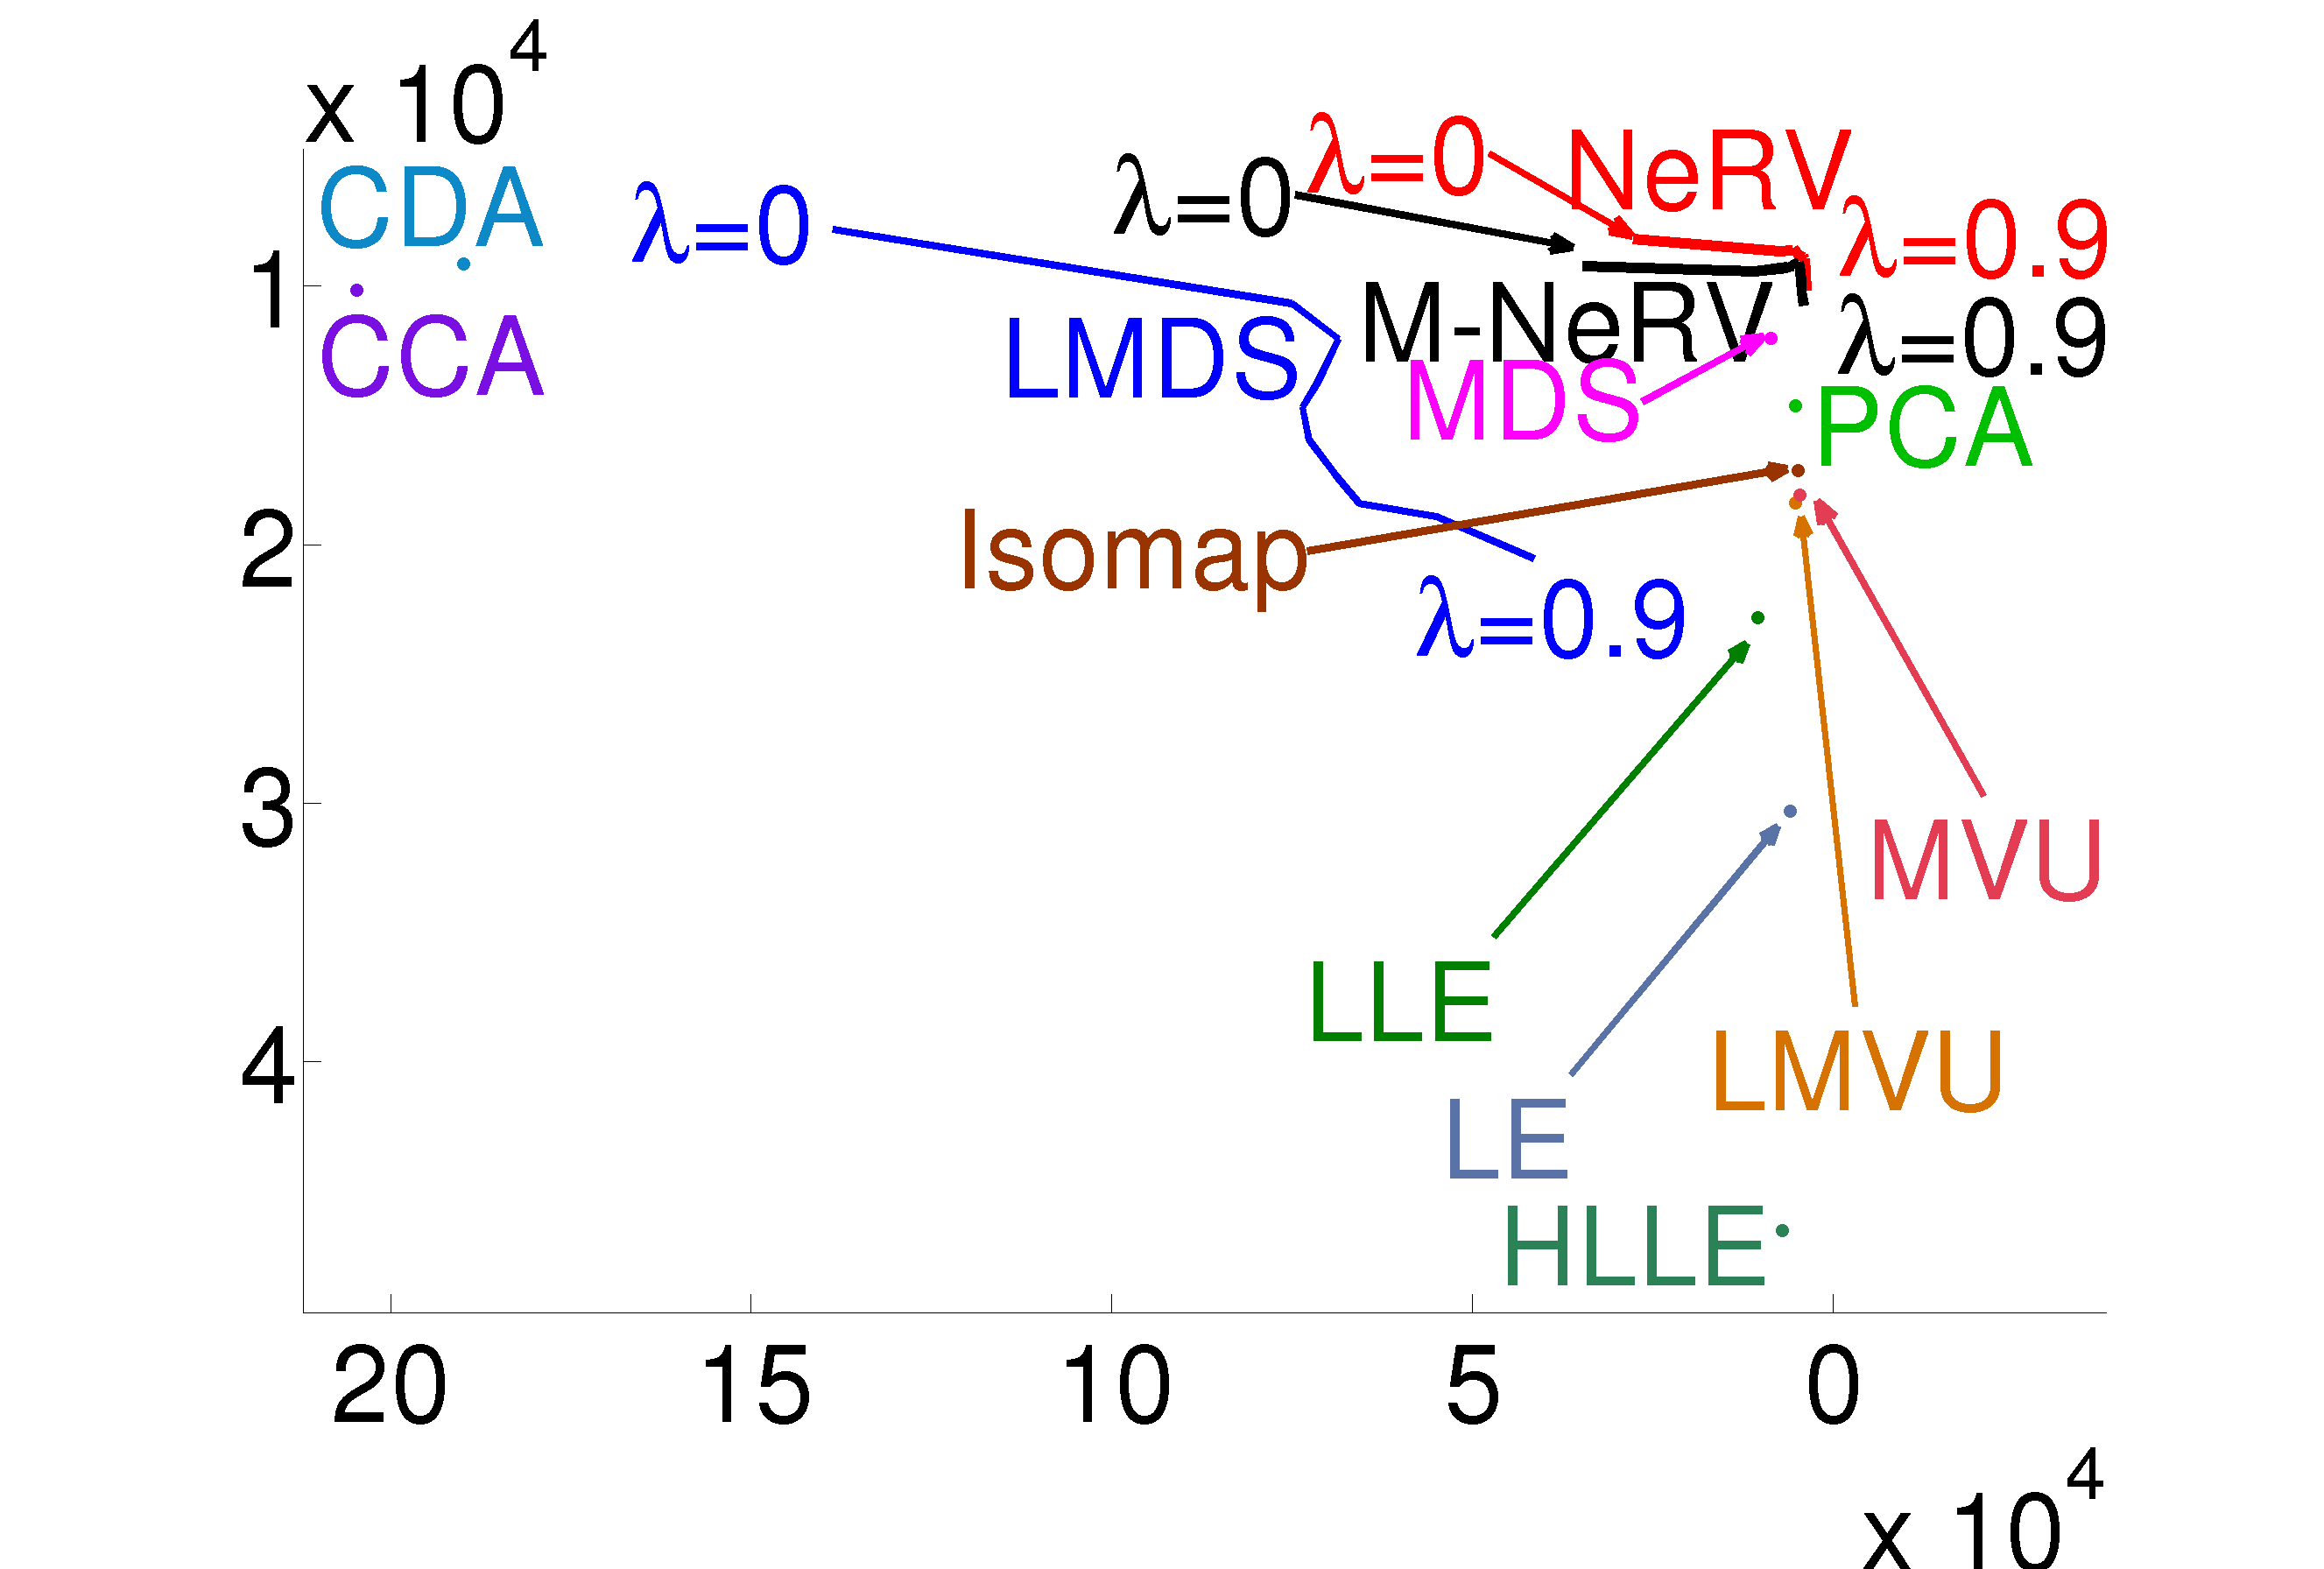
\includegraphics[width=0.5\textwidth]{figures/smoothed-precision-recall-hiiri.pdf}} 
\end{tabular}
\caption{Mean smoothed recall vs. mean smoothed precision for different methods. Best methods are located top-right. Mouse Gene Expression data set: gene expression profiles from different mouse tissues.}
\end{figure}
\end{frame}


\begin{frame}{Experiments: comparison with other NLDR methods}
\begin{figure}[!htb]
\captionsetup[subfigure]{labelformat=empty}
\centering
\begin{tabular}{cc}
\subfloat[Gene Expression Compendium]{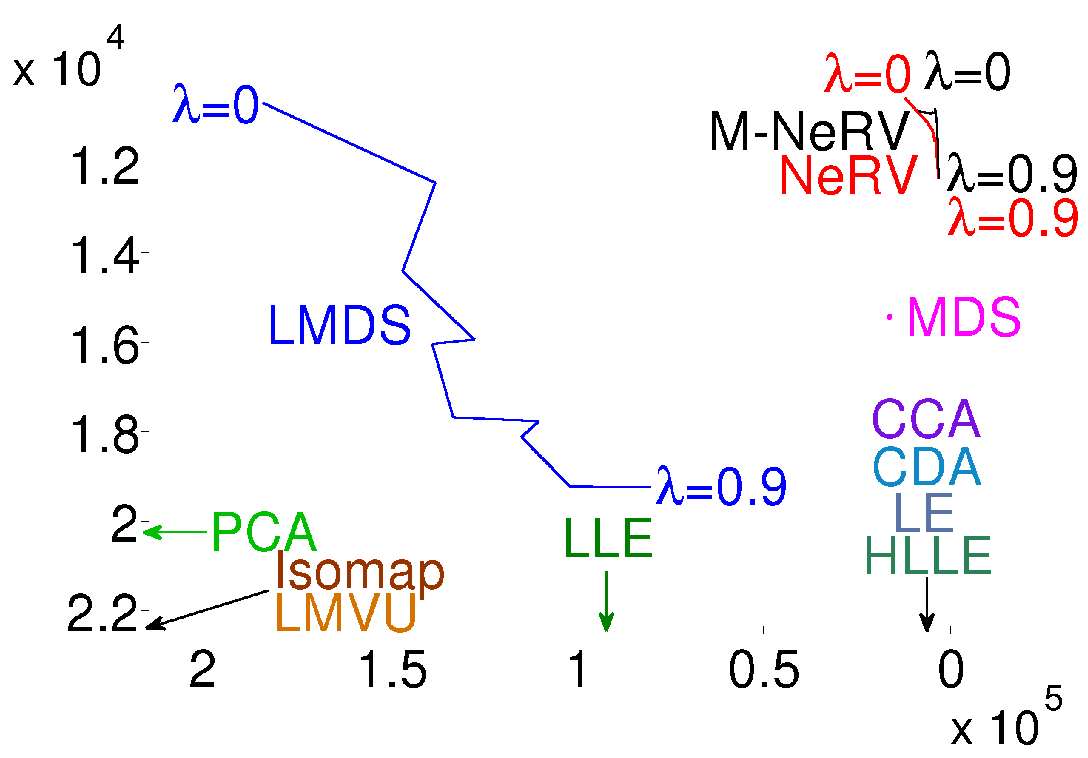
\includegraphics[width=0.5\textwidth]{figures/smoothed-precision-recall-segal-1-t.pdf}} &
\subfloat[Sea-water Temperature Time Series]{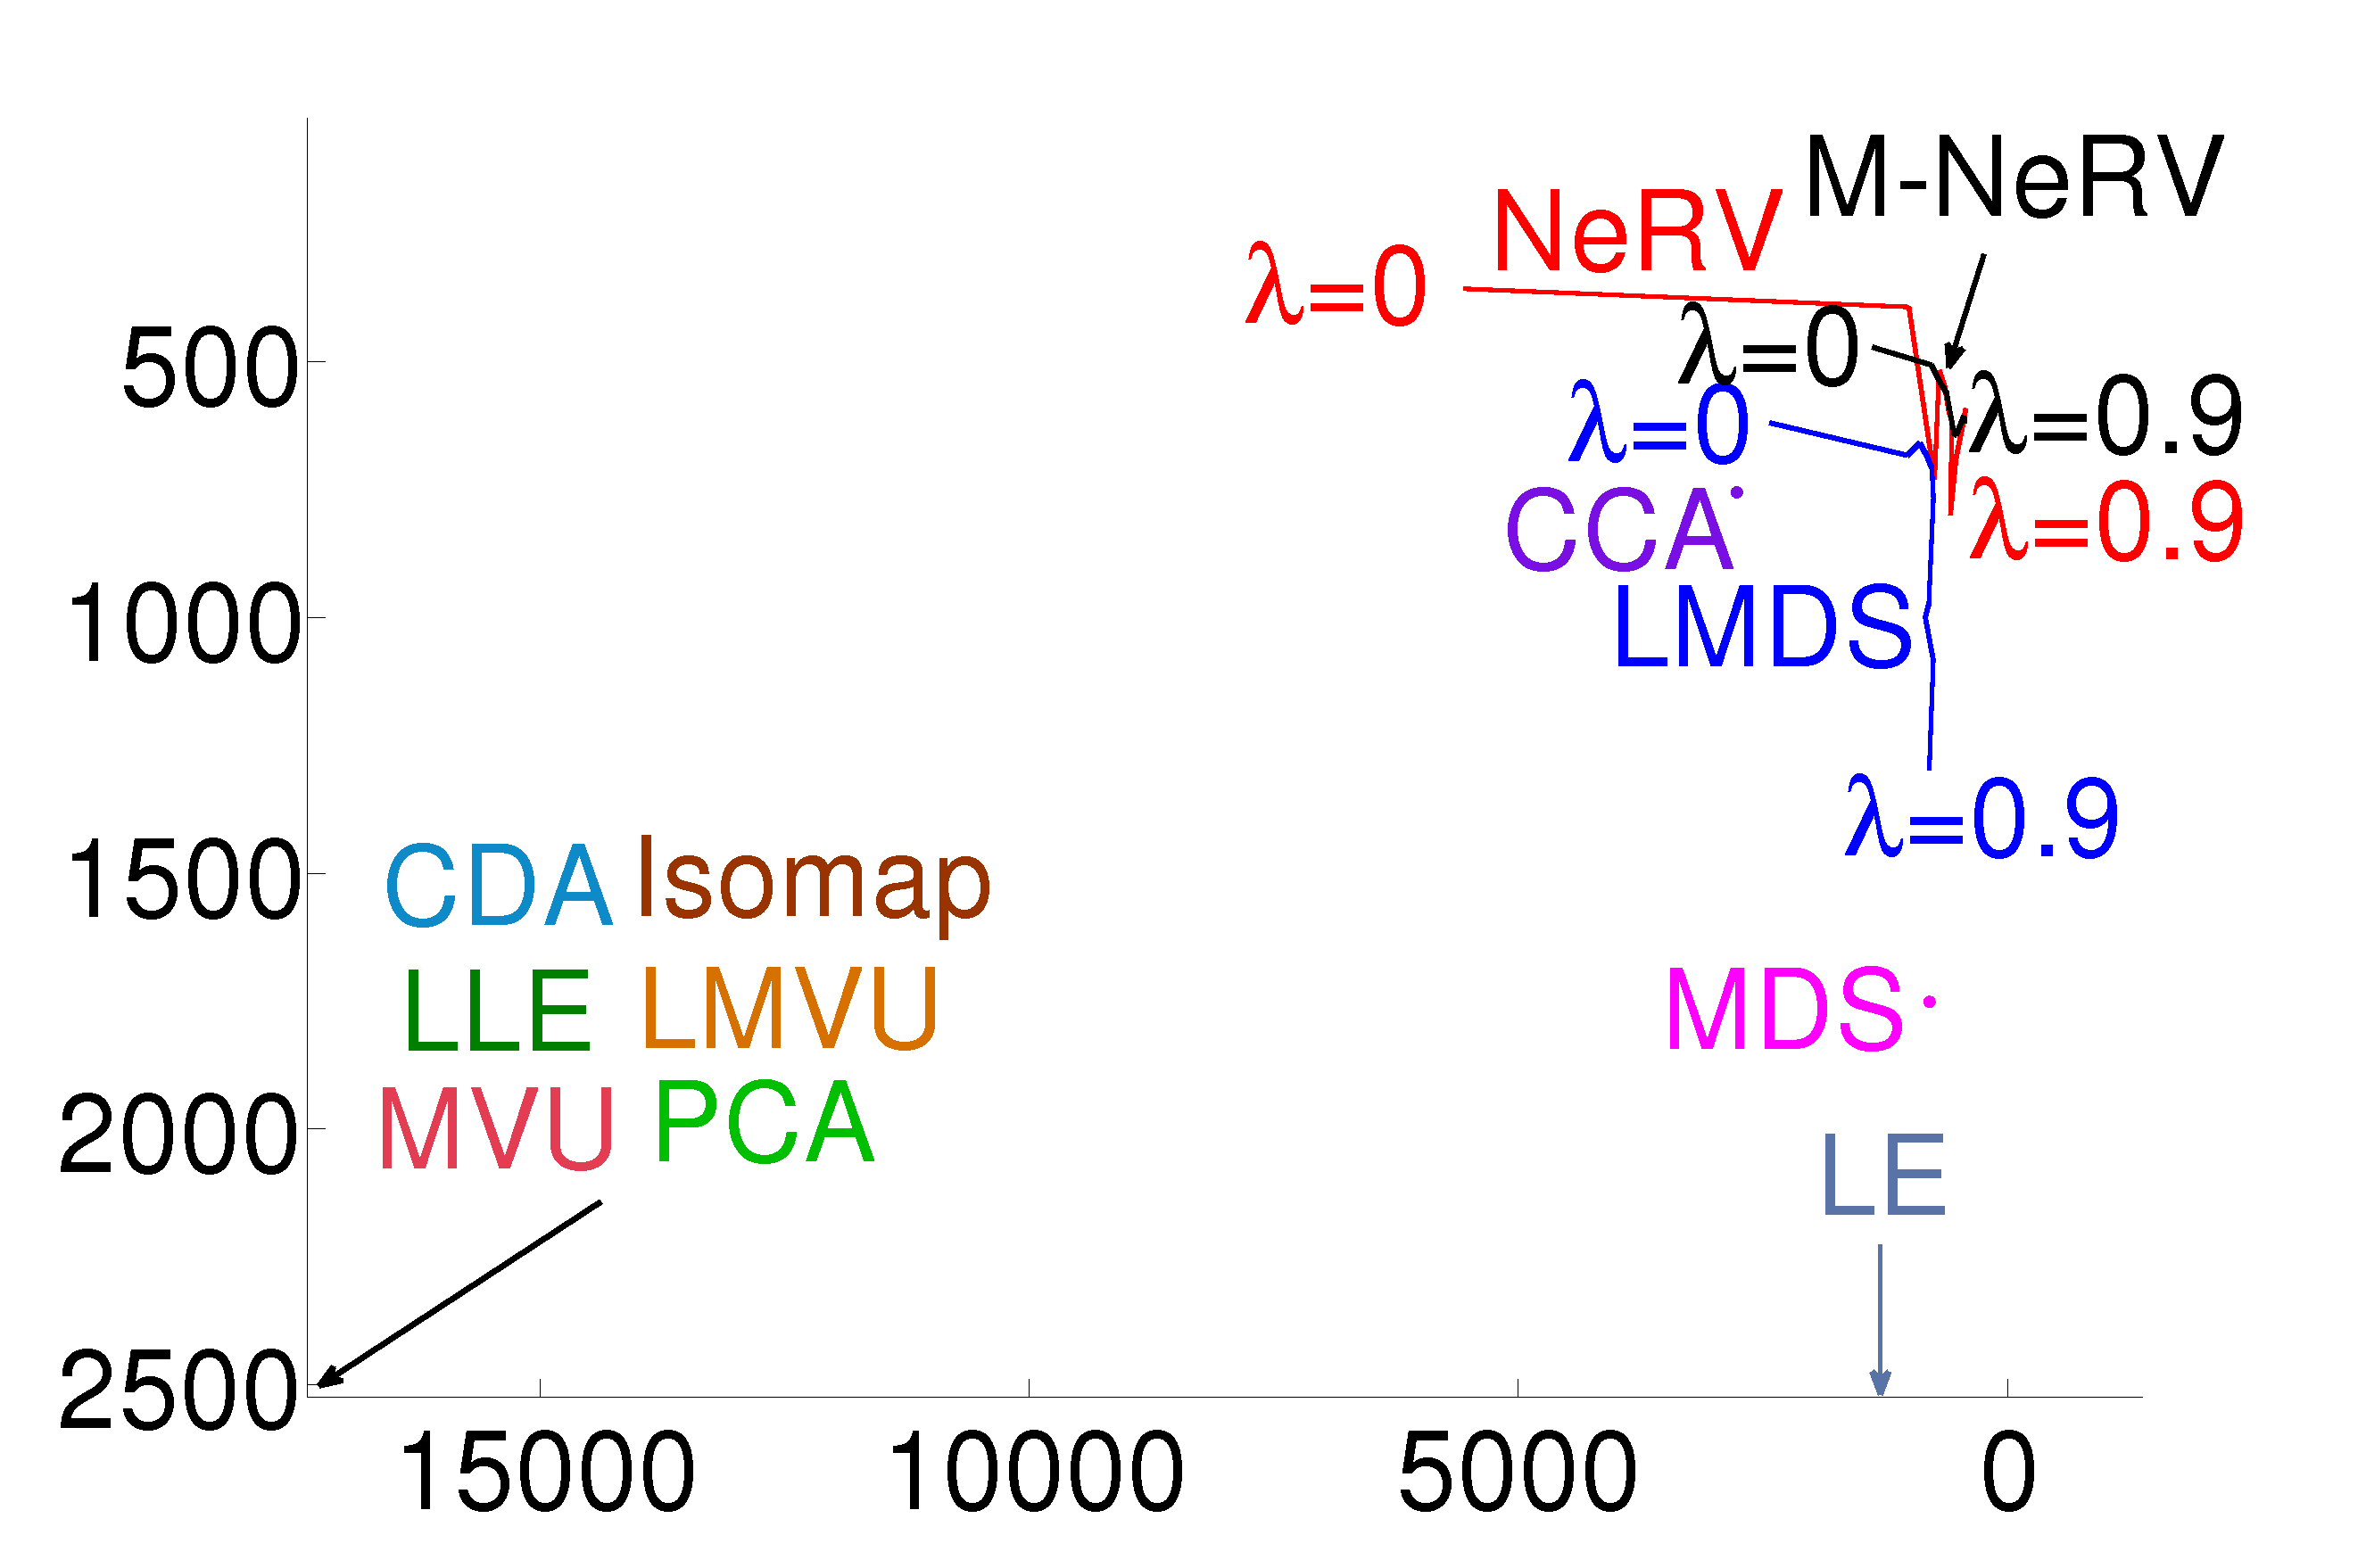
\includegraphics[width=0.5\textwidth]{figures/smoothed-precision-recall-estsp52.pdf}} 
\end{tabular}
\caption{Gene Expression Compendium data set: human gene expression arrays; Sea-water Temperature Time Teries data set: a time series of weekly temperature measurements of sea water over years.}
\end{figure}
\end{frame}


\begin{frame}{Conclusion}
\begin{enumerate}
\item NeRV is a method that is already known to perform very well in experiments of comparison with other methods. In this paper we address the speed of learning;
\item We introduced a multiplicative update rule for the information retrieval based visualization method Neighbor Retrieval Visualizer (NeRV);
\item It needs no user-assigned learning rate parameter or line search, but yields strong speedup over original NeRV and maintains state of the art performance, in terms of qualitative appearance of visualizations and quantitative information retrieval performance measures.
\end{enumerate}
\end{frame}
\end{document}